\documentclass{report}
\usepackage{graphicx}
\usepackage{sidecap}
\usepackage{hyperref}
\usepackage[margin=3cm]{geometry}
\usepackage{listings}
\usepackage{xcolor}
\usepackage{svg}
\usepackage{tikz}
\usepackage{amsmath}


% Define MATLAB style
\lstdefinestyle{MATLABstyle}{
    language=Matlab,               % Set language to MATLAB
    basicstyle=\ttfamily\small,    % Basic font style
    keywordstyle=\color{blue},     % Keywords in blue
    commentstyle=\color{green!60!black}, % Comments in dark green
    stringstyle=\color{red},       % Strings in red
    numbers=left,                  % Line numbers on the left
    numberstyle=\tiny,             % Style of line numbers
    stepnumber=1,                  % Line numbers for every line
    numbersep=10pt,                % Space between line numbers and code
    backgroundcolor=\color{gray!10}, % Light gray background
    frame=single,                  % Draw a frame around the code
    rulecolor=\color{black},       % Frame border color
    breaklines=true,               % Line breaking for long lines
    breakatwhitespace=true,        % Break at whitespace if possible
    showspaces=false,              % Do not show spaces as special characters
    showstringspaces=false,        % Do not mark spaces in strings
    tabsize=4,                     % Number of spaces per tab
}


\title{%
    Rubik's Cube Automatic Solver \\
    \medskip \\
    \large Mechatronic System Design Project \\
    \large University of Pisa}
\author{Alessandro Palla \\
        Leonardo Bove}
\date{December 2024}

\begin{document}

\maketitle
\newpage
\tableofcontents

\chapter{Introduction}
The code and STL files of this project can be found on \href{https://github.com/leonardobove/rubik_solver_robot/tree/main}{GitHub}.
\section{Project Objectives}

The objective of the project is to read and solve a 3x3 Rubik's cube using an automatic robot, programmed via MATLAB and Simulink.
\newline
Robot management is handled by the NXP S32K144EVB-Q100
microcontroller thanks to Simulink's Model-Based Design Toolbox for S32K1xx.


\section{Requirements}

In order to properly control the robot, we faced the following challenges:
\begin{itemize}
    \item Manage the communication between PC and microcontroller through PIL execution.
    \item Acquisition of colors from the cube's faces using a webcam.
    \item Control of four servo motors.
\end{itemize}

\subsection{Hardware}
In the project, the following hardware has been used:
\newline
\begin{itemize}
    \item The NXP S32K144EVB-Q100.

        \begin{center}
        \includegraphics[width=0.4\textwidth]{images/Requirements/s32k_no_bg.png} 
        \end{center}
   
    \item A 3D printed support (PLA), downloaded from an other project found on \href{https://www.thingiverse.com/thing:3826740}{thingiverse}.

        \begin{center}
        \includegraphics[width=0.4\textwidth]{images/Requirements/supporto_3D_noBg.jpg} 
        \end{center}

     \item 4 Miuzei MZ996 180° servo motors controlled by a PWM with a duty-cycle, whose values lay in the range between 0.025 and 0.125. The datasheet is available \href{https://www.electronicoscaldas.com/datasheet/MG996R_Tower-Pro.pdf?srsltid=AfmBOor49yoIi3HG1Glu8xAof5r7fDnHv_RtM06DaJG2pPgA_Chr45Gq}{here}.

        \begin{center}
        \includegraphics[width=0.3\textwidth]{images/Requirements/servo_motor_no_bg.jpg} 
        \end{center}

     \item The Braccio Shield v4 from \href{https://store.arduino.cc/products/tinkerkit-braccio-robot?srsltid=AfmBOoqExbUeCwcXCfRaFAXlicvBgPllll6ozcArsreP7fObxQhmhGch}{Arduino robotic arm Tinkerkit}, a 5V Power board where the 4 servo motors are connected. This object, connected to the power supply, is necessary because of the limited available power of the PC's USB port. The schematic can be found \href{https://content.arduino.cc/assets/Braccio-Shield-V1.pdf}{here}.

        \begin{center}
        \includegraphics[width=0.3\textwidth]{images/Requirements/arduino_braccio_shield_no_bg.png}
        \end{center}

    \item A webcam for scanning the cube's faces.

        \begin{center}
        \includegraphics[width=0.2\textwidth]{images/Requirements/webcam_no_bg.png}
        \end{center}
        
\end{itemize}


\subsection{Software}
 To use the NXP S32K144EVB-Q100 functions, Matlab and Simulink needed the following extension:
\begin{itemize}
    \item NXP Support Package S32K1xx 
    \item Model-Based Design Toolbox for S32K1xx
    \item Stateflow
    \item Simulink Embedded Coder
    \item Simulink Test
    \item Simulink SIL/PIL Manager
\end{itemize}
In addition, two more toolboxes have been added: the \textbf{MATLAB Support Package for USB Webcams} with the aim of managing the webcam, and the \textbf{Rubik's Cube Simulator and Solver} toolbox. The latter was of significant importance for the project, because it allowed us to generate a digital model of the cube (see section \ref{sec:rub-cub-mod}) and to implement the \textit{Thistlethwaite 45} resolution algorithm on MATLAB.

\section{Electrical Wiring}
The \textit{Arduino Braccio Shield} can be directly mounted on top of the NXP board, which has an Arduino compatible pin header. In order to supply the servo motors with the 5V external power supply connected to the shield, it is necessary to enable it, by setting to a high logic level the PTB3 NXP GPIO, which corresponds to the D12 digital pin on the Arduino compatible pin header of the shield. This is shown in figure \ref{fig:shield-enable}.

\begin{figure}[h]
    \centering
    \includegraphics[width=0.5\linewidth]{images/Requirements/shield_enable.png}
    \caption{Shield enabling}
    \label{fig:shield-enable}
\end{figure}

Unfortunately, the servo motors pin headers on the shield have a different pinout (5V-SIGNAL-GND) compared to the one of the motors (SIGNAL-5V-GND), as you can see in figure \ref{fig:shield-wiring}. For this reason, instead of re-wiring the motors, male-female jumper wires were used to connect the right lines.

\begin{figure}[h]
    \centering
    \includegraphics[width=0.5\linewidth]{images/Requirements/braccio_shield_wiring.png}
    \caption{Servo motors wiring to the driver shield.}
    \label{fig:shield-wiring}
\end{figure}

In particular, the following connections were made:
\begin{itemize}
    \item The left arm motor was connected to the M1 connector, whose signal line corresponds to the \textbf{PTB4} PWM output on the NXP board.
    \item The left grip motor was connected to the M2 connector, whose signal line corresponds to the \textbf{PTB5} PWM output on the NXP board.
    \item The right arm motor was connected to the M3 connector for the power supply, but, given that its signal line didn't lead to any PWM output on the NXP board, its PWM signal input was directly connected to the \textbf{PTD15} PWM output of the board.
    \item The right grip motor was connected to the M4 connector for the power supply, but, for the same reason as the previous one, its PWM signal input was directly connected to the \textbf{PTD16} PWM output of the board.
\end{itemize}

For the correspondence between the shield signal lines and the GPIO pins on the NXP board, the following schematic was used (\ref{fig:shield-pinout}):

\begin{figure}[h]
    \centering
    \includegraphics[width=0.75\linewidth]{images/Requirements/shield_pinout.png}
    \caption{Arduino Braccio shield v4 pinout}
    \label{fig:shield-pinout}
\end{figure}


\chapter{System Description} 
\section{PIL System}    \label{sec:pil-sys}
The system was implemented using a \textbf{PIL} (\textit{Processor-in-the-Loop}) execution. This means that the system is subdivided into different models, some of which are directly run by the MATLAB engine on the PC whereas others are used to generate C source code, which is compiled and downloaded onto the target hardware (in this case the S32Kxx microcontroller); afterwards, the user can simultanously run the code on the target and the other models on the PC through a Simulink Processor-in-the-Loop Simulation, which enables a UART communication between the two hardwares, allowing data exchange and verification.

This execution mode is generally used to test an embeddable model on the target device, while the PC models the environment where the microcontroller will be deployed, without the need of testing it directly in the real environment. This helps in testing the embedded software faster and without compromising the real environment, which can sometimes result in dangerous consequences. In this case, the PIL simulation environment is actually used as part of the under-test system, for the reasons that will be explained in the next subsection.

\subsection{Pros and Cons of PIL Simulation}
The choice of the PIL simulation was pursued for the following advantages:
\begin{itemize}
    \item \textbf{Delegation of complex tasks} to the PC: some functions, e.g. the webcam acquisition and the Rubik's cube solver algorithm, are easier to implement on the MATLAB environment because they were already available as application libraries or they would have required a computation effort that made it not implementable on an embedded system.
    \item \textbf{Easy debugging} and signal \textbf{logging}: Simulink PIL simulation provides a real-time data viewer and allows to compare logged signals from different runs of the simulation.
    \item \textbf{Simplified} set-up of the communication interface between PC and microcontroller via \textbf{UART}: Simulink automatically includes APIs in the generated embedded code that allow to exchange data via UART.
    \item Highly \textbf{customizable user interface}: in the simulation enviroment, there are many dashboard blocks that allow the user to easily interact with the model deployed on the target hardware.
\end{itemize}

On the other hand, this choice implies some disadvantages:
\begin{itemize}
    \item Not perfect synchronization between PC and microcontroller: due to the overhead introduced by the MATLAB engine, sometimes there can be a pace error between the PC and the microcontroller simulation times.
    \item UART interface not optimized: even though it is easier to set-up for complex data exchange, it is not optimized. This problem can be overcome by defining a custom UART data exchange protocol.
    \item Impossibility to realize a stand-alone system: this problem can be solved by using a more powerful embedded system (e.g. a \textit{Raspberry Pi}), so that the webcam management and solver algorithm can be implemented directly on the target hardware, making it independent from the MATLAB engine.
\end{itemize}

\subsection{System Overview}
In figure \ref{fig:overall_system} is presented the overall system.

\begin{figure}[h]
    \centering
    \includegraphics[width=1.0\linewidth]{images/PIL_system/test_harness.jpg}
    %\includesvg[width=1.0\linewidth]{images/PIL_system/PIL_system}
    \caption{Overall system overview}
    \label{fig:overall_system}
\end{figure}

This view is taken from the Simulink \textbf{Test Harness} manager, because, for the way the PIL simulation is originally thought, the actual DUT is the model that will be implemented on the microcontroller, while the other non-embedded blocks are built in the testing environment.

We can distinguish four main blocks in the system:
\begin{itemize}
    \item \textbf{Cube Actuator}: this block models the actuator for the motors and the main finite-state machine of the system and this is the model that will be embedded into the microcontroller.
    \item \textbf{Webcam Manager}: this block is responsible for the webcam management and the cube's colors acquisition. It is run by the MATLAB interpreter.
    \item \textbf{Rubik's Cube Model}: this block manages the virtual model of the physical cube and the sequence of solving moves.
    \item \textbf{User Interface}: this area implements the user interface using blocks from the \textit{Simulink Dashboard} resources.
\end{itemize}

As we can see, these blocks communicate through Simulink signals, which are delivered to the embedded model as well, thanks to the PIL simulation UART interface. Exchange of data happens also through \textit{Data Store Memory} blocks (global variables) which are written by some models and read by others.

The two execution times are set to be equal (i.e. 1 second on the PC equals to 1 second on the microcontroller) and the models' tick time is set to 0.1 seconds.

\subsection{MATLAB System Block} 
This block was used to implement both the \textit{Webcam Manager} and the \textit{Rubik's Cube Model}. It allows to implement algorithms using the MATLAB scripting language inside the Simulink environment. Moreover, it lets the user decide whether to generate source C code from it or to run it using the interpreter: the latter was the option that was helpful for our system.

Other relevant features of this block are that it allows to define state variables, to keep track of the current state of the subsystem, and the user can define an arbitrary number of input and output ports. Unfortunately, output ports were not used, because, apparently, they forced the system to be compiled into C code, especially if those output signals were connected to the \textit{Cube Actuator} model. To solve this issue, we opted for system global variables (\textit{Data Store Memory}), written by the two MATLAB Block Systems and read by the other embedded model.

\medskip

The software implementation of this kind of block is made by means of a particular class, called \textbf{System object}. The default System object template is reported in \ref{code:system_obj}.

\begin{lstlisting}[
style=MATLABstyle,
caption={System object template},
label=code:system_obj
]
classdef untitled < matlab.System
    % untitled Add summary here
    %
    % This template includes the minimum set of functions required
    % to define a System object with discrete state.

    % Public, tunable properties
    properties

    end

    properties (DiscreteState)

    end

    % Pre-computed constants
    properties (Access = private)

    end

    methods (Access = protected)
        function setupImpl(obj)
            % Perform one-time calculations, such as computing constants
        end

        function y = stepImpl(obj,u)
            % Implement algorithm. Calculate y as a function of input u and
            % discrete states.
            y = u;
        end

        function resetImpl(obj)
            % Initialize / reset discrete-state properties
        end
    end
end
\end{lstlisting}

As we can see, the user can define \texttt{properties} that can be used to store state variables: unfortunately, their type can only be logical, numerical or an enumeration. These \texttt{properties} get initialized inside the \texttt{resetImpl} function. The main body of the system is the \texttt{stepImpl} function, which is executed at every simulation tick. The user can define input and output signals for the system, just by changing the input and output arguments of this function. From here, any MATLAB script can be called, gaining access to all the Simulink toolboxes.

\section{Cube Actuator}
The block \textbf{Cube Actuator} is the heart of the system, which is embedded in the NXP board.
As we can see from figure \ref{fig:cub-act}, the model was implemented on Simulink, using the \textit{NXP's Model Based Design} toolbox. Here, we can distinguish four main blocks.
The first is the \textbf{Stateflow}, which will be described in the next section. Its output is a \textbf{microcode} composed of four digits, one for each servo motor.
\begin{itemize}
 \item first digit [0, 1]: open/close left grip;
 \item second digit [0, 1]: open/close right grip;
 \item third digit [0, 1, 2]: set left arm to 90/0/180 degrees
 \item  fourth digit [0, 1, 2]: set right arm to 90/0/180 degress
\end{itemize}

The following block is the \textbf{Cube Operation Decoder}, which takes as input the microcode and separates it into four different outputs. These are fed to the \textbf{Actuate Servos}, which converts the numbers in the corresponding duty-cycle values for the servos control. This way, a discrete positions actuation is implemented.

The duty-cycle values are assigned as input of the \textbf{NXP PWM Config block}, which generates the C source code to control the PWM registers on the board.

    \begin{figure}[h]
    \centering
    \includegraphics[width=1.0\linewidth]{images/Cube_actuator/cube_actuator.jpg}
    \caption{Cube Actuator blocks}
    \label{fig:cub-act}
    \end{figure}
    
\subsection{Stateflow}
Looking at the Stateflow, it is possibile to distinguish two macro groups: the \textbf{control section} and the \textbf{execution section}. The control section manages the operational phases of the robot, while the execution section sequentially executes the commands to perform a move on the cube.

\begin{figure}[h]
    \centering
    \includegraphics[width=1.0\linewidth]{images/Cube_actuator/state_flow.png}
    \caption{Stateflow}
    \label{fig:sta-flo}
\end{figure}

\subsubsection{Control Section}
As you can see in figure \ref{fig:sta-flo-con}, the control section is composed by 5 states:
\begin{itemize}
\item \textbf{wait\_cube}: all local variables are initialized, the output \texttt{reset} is set to 1, initializing all variables in the \textit{Webcam Manager} and in the \textit{Rubik's Cube Model} (see sections \ref{sec:web-man} and \ref{sec:rub-cub-mod}). The \texttt{microcode} sent as output in this state is 1000, therefore one of the pliers is open and the other is closed. In this way, the user can easily place the cube on the arms. The cube has to be placed with the face having the red central tile in front of the webcam, and the face with the white central tile on the top.
\item \textbf{webcam\_alignment}: \texttt{reset} is set to 0 and will keep this values for all the other states. The \texttt{microcode} changes to 1100, closing both pliers. The output \texttt{webcam\_alignment\_trig} is set to 1, starting the thread \texttt{webcam\_alignment}, see \ref{sub_sec:web-ali}.
\item \textbf{read\_cube}: in this state the output \texttt{webcam\_alignment\_trig} is set to 0, the instantiated states are activated and they rotate the cube, in order to sequentially read the 6 faces, starting from the face with the red central cell, followed by blue, orange, green, white and yellow. At the end of the reading sequence, the cube is taken back to the original position. This is possible thanks to the instantiated states which sequencially changes every 2~sec, allowing the \texttt{microcode} to change accordingly. Moreover, once the next face is aligned with the webcam, the output \texttt{read\_face\_trig} is set to 1, triggering the acquisition of the colors of one face. Afterwards the user can decide to accept the acquired colors, retake a picture or manually load the face configuration. See \ref{sub: fac-col-acq} for more details.
\item \textbf{solve\_cube}: this is the interface between the execution and control states. The \texttt{microcode} is set again to 1100 while the output \texttt{read\_done}, if the user does not press any button, is set to 1. This lets the \texttt{Rubik's Cube Model block} to update the \texttt{current\_move\_idx}, in order to process the next move in the execution states. Before moving to the execution states, \texttt{read\_done} is set again to 0. See section \ref{sec:rub-cub-mod}.
\item \textbf{waiting}: the user can decide to pause the cube's solving by going inside this state and restart the execution at any time.
\end{itemize}

\begin{figure}[h]
    \centering
    \includegraphics[width=1.0\linewidth]{images/Cube_actuator/stateflow_control.png}
    \caption{Control section of the Stateflow}
    \label{fig:sta-flo-con}
\end{figure}

\subsubsection{State connections} 
In order to move from one state to the other, some specific conditions need to be verified. Before explaining how state connections work, it is important to highlight that the stateflow transitions that depend on SW2 or SW3 button inputs are \textbf{sensitive to only the rising edge} of the associated input signal.

\bigskip

Starting from the \texttt{wait\_cube} state, the user can close the pliers and go to \texttt{webcam\_alignment} by pressing the SW2 button. After this initial condition, SW2 will be the \textbf{reset} button for all the other states, allowing to come back to \texttt{wait\_cube} and opening one of the pliers. The reset cannot happen during the execution of a single move.

Once the user has completed the webcam alignment, by pressing SW3 the cube's reading starts, thus going into the associated state. If, however, the input constant \texttt{skip\_cube\_read} is set to 1, it means that the user does not want to scan the cube, inserting it manually instead, see \ref{sub: fac-col-acq}. In this case by pressing SW3, the next state will be directly \texttt{solve\_cube}.

\texttt{read\_cube} state goes to \texttt{solve\_cube} once the last face has been read. In order to accept a cube's face scan and continue with the acquisition, the user has to press SW3. If the face was manually loaded, SW3 is still necessary to proceed with the acquisition.

The connection between the execution states and \texttt{solve\_cube} state is possible thanks to the input \texttt{execute\_move}, which is set to 1 by the \textit{Rubik's Cube Model}, see \ref{sub:sol-mov-man}. 

When the \textit{Rubik's Cube Model} sets to 1 the global variable \texttt{execute\_move}, the system goes into one of the execution state, doing a move of the cube's solving. The move to be executed is specified by the \texttt{next\_move} input, which consists of an array of two characters. Moreover, from \texttt{solve\_cube} it is possible to switch to the \texttt{waiting} state if SW3 button is pressed or if the local variable \texttt{pause} is equal to 1.

From \texttt{waiting} if the user presses again SW3, the execution is resumed, going back to \texttt{solve\_cube} state.

\subsubsection{Execution Section}
Each of the 18 states in this section corresponds to a move to be performed. 

When the global variable \texttt{execute\_move} is set to 1, the stateflow moves from \texttt{solve\_cube} to the execution state specified by \texttt{next\_move}.
Each execution state is composed of multiple sub-states, which change the output \texttt{microcode} in order to rotate or modify the cube.

At the end of the last cube's operation of one execution state, the stateflow goes back to \texttt{solve\_cube}. This process is repeated until the end of the solution moves.

Besides, every state contains a pause and reset condition. If 
the user presess SW3, the local variable \texttt{pause} is set to 1; similarly pressing SW2 the local variable \texttt{reset\_status} is set to 1. In this way it is possible to go to \texttt{waiting} or \texttt{wait\_cube} states directly from \texttt{solve\_cube} checking these local variables, as soon as the current move is finished.

\subsection{Cube Operation Decoder and Actuate Servos} \label{sec:motor_pos_decoder}
To convert the \texttt{microcode} in 4 distinct inputs, a MATLAB function with the following body has been used:
\begin{lstlisting}[
style=MATLABstyle,
caption={Cube\_operation\_decoder},
label=code:decoder
] 
function [move_bl, move_tl, move_br, move_tr] = cube_operation_decoder(cube_operation)
x1 = int32(mod(cube_operation/1000, 10));
x2 = int32(mod(cube_operation/100, 10));
x3 = int32(mod(cube_operation/10, 10));
x4 = int32(mod(cube_operation, 10));

move_tl = x1;
move_tr = x2;
move_bl = x3;
move_br = x4;
\end{lstlisting}

\bigskip

After that, the outputs are converted into the corresponding duty-cycle values with another MATLAB function:
\begin{lstlisting}[
style=MATLABstyle,
caption={Actuate\_Servos},
label=code:act-serv
] 
function [BR, TR, BL, TL] = actuate_servos(move_bl, move_tl, move_br, move_tr)

min_duty = 0.025;
max_duty = 0.125;

duty_0_deg = min_duty;
duty_grip_open = min_duty + (max_duty-min_duty)/3;
duty_grip_closed = min_duty + (max_duty-min_duty)/14; 
duty_90_deg = min_duty + (max_duty-min_duty)/2;
duty_180_deg = max_duty;


duty_offset_left_arm = (max_duty-min_duty)/30;
duty_offset_right_arm = 0;

switch (move_tl)
    case 0                  % Open left grip
        TL = duty_grip_open;
    case 1                  % Close left grip
        TL = duty_grip_closed;
    otherwise               % Open left grip
        TL = duty_grip_open;
end

switch (move_tr)
    case 0                  % Open right grip
        TR = duty_grip_open;
    case 1                  % Close right grip
        TR = duty_grip_closed;
    otherwise               % Open right grip
        TR = duty_grip_open;
end

switch (move_bl)
    case 0                  % Left arm straight
        BL = duty_90_deg + duty_offset_left_arm;
    case 1                  % Left arm at 90° clockwise
        BL = duty_0_deg + duty_offset_left_arm;
    case 2                  % Left arm at 90° counter-clockwise
        BL = duty_180_deg + duty_offset_left_arm;
    otherwise
        BL = duty_90_deg + duty_offset_left_arm;
end

switch (move_br)
    case 0                  % Right arm straight
        BR = duty_90_deg + duty_offset_right_arm;
    case 1                  % Right arm at 90° clockwise
        BR = duty_0_deg + duty_offset_right_arm;
    case 2                  % Right arm at 90° counter-clockwise
        BR = duty_180_deg + duty_offset_right_arm;
    otherwise
        BR = duty_90_deg + duty_offset_right_arm;
end

\end{lstlisting}
It is possible to notice that, in order to compensate for alignment errors between the two motors and therefore to be able to fine-tune the motors positions, two \textbf{offset} values were added.

\section{Webcam Manager} \label{sec:web-man}
This block is responsible for the webcam management, thanks to \textit{MATLAB Support Package for USB Webcam}. The system block is presented in figure \ref{fig:webcam_manager_block}.

\begin{figure}[h!]
    \centering
    %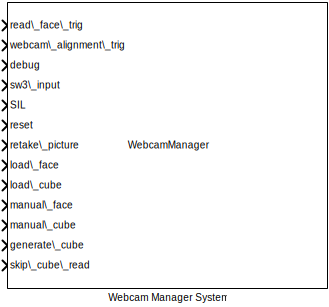
\includegraphics[width=0.5\linewidth]{images/webcam_manager/webcam_manager_block.png}
    \includesvg{images/webcam_manager/webcam_manager_block}
    \caption{Webcam Manager System Block}
    \label{fig:webcam_manager_block}
\end{figure}

The tasks performed by this system are the following:
\begin{itemize}
    \item \textbf{Webcam alignment}
    \item \textbf{Face colors acquisition}
\end{itemize}

These tasks are triggered by the rising edge of signals coming from the \textit{Cube Actuator}. The rising edge detection is implemented using state variables that store the previous value of the respective input. For example, the state variable \texttt{webcam\_alignment\_trig\_status} is updated every tick with the current value of the corresponding input, \texttt{webcam\_alignment\_trig}: at the next simulation tick, if \texttt{webcam\_alignment\_trig == 1} and \texttt{webcam\_alignment\_trig\_status == 0}, this means that a rising edge on that signal has occurred.

The \texttt{reset} input is likewise controlled by the \textit{Cube Actuator} and triggers an immediate reset of all the state variables.

\subsection{Webcam Alignment} \label{sub_sec:web-ali}
When a rising edge on the signal \texttt{webcam\_alignment\_trig} is detected, the MATLAB script \texttt{webcam\_alignment} is started: this script opens the connected USB webcam, displays a video preview of what the webcam sees and prints over the frames nine equally spaced red circles which form a square, so that the user can adjust the position of the webcam, in order to align the circles with the nine tiles of a single Rubik's cube face (see figure \ref{fig:webcam_align_view}). This way the face colors acquisition will correctly read the colors in the middle of each tile.

\begin{figure}[h!]
    \centering
    \includegraphics[width=0.5\linewidth]{images/webcam_manager/alignment.jpg}
    \caption{Webcam alignment view}
    \label{fig:webcam_align_view}
\end{figure}

Since the script continuously outputs the preview from the webcam, to make it easier for the user to perform the alignment, in order not to pause the whole simulation, it has to be executed on a different background thread. This is accomplished my means of the MATLAB function \texttt{parfeval}.

\begin{lstlisting}[
style=MATLABstyle,
caption={Background thread execution},
label=code:bg_thread
]
if webcam_alignment_trig == 1 && obj.webcam_alignment_trig_status == 0
    obj.webcam_alignment_process = parfeval(@webcam_alignment, 0);   % Enable webcam alignment in a separate thread
    obj.alignment_in_progress = true;
\end{lstlisting}

As we can see in \ref{code:bg_thread}, \texttt{parfeval} is called with second argument set to 0, which tells the interpreter that no output is expected from the new thread. \texttt{parfeval} returns a \textit{future object}, which is assigned to the state variable \texttt{webcam\_alignment\_process}. It can be later used to retrieve the thread outputs, if any, and to terminate the background thread using the function \texttt{cancel}, as soon as the alignment is completed and approved by the user by pressing the SW3 button.

\subsection{Face Colors Acquisition} \label{sub: fac-col-acq}
When a rising edge on the signal \texttt{read\_face\_trig} is detected, the \texttt{get\_face\_colors} script is triggered. This time there is no need of a background thread, since the script is non-blocking. It opens the webcam, takes a picture and computes nine RGB color codes by averaging the RGB values inside each of the nine circle areas used during the webcam alignment phase. These nine RGB color codes are compared with hardcoded RGB ranges, each of which corresponds to one of the six possible colors on the cube. Each color correspond to a different integer: red is 1, blue is 2, orange is 3, green is 4, white is 5 and yellow is 6. \texttt{get\_face\_colors} returns a 3x3 matrix containing the color integer codes detected for each tile. If no color is recognized, the matrix element corresponding to that tile is set to 0. If the \texttt{debug} input port of the system is set to 1, this script will also return the RGB average colors that have been acquired for debug and calibration purposes.

Once the acquisition is completed, the webcam must be closed, since it is not possible to store its handler in any state variable of a MATLAB System Block, and the face colors matrix is analyzed: if any of the elements is 0 (undefined color), the user is notified through the simulation log and it is possible to re-take the picture by pressing the \textit{Re-take picture} button; otherwise, the user can approve the read colors (errors during acquisition can occur) by clicking the SW3 button and the face is loaded onto the global 3x3x6 \texttt{cube} matrix, that holds the color configuration of the whole cube during the simulation. When a face is approved, the global variable \texttt{read\_done} is set to 1 (and reset to 0 later on): this flag is read by the \textit{Cube Actuator}, which now can proceed and rotate the cube, in order to present to the webcam the following face to be read.

\medskip

Due to bad light environments, it can happen that some colors of a face are hard to read. In this case, the user can manually load the color configuration of the current face through the user interface (see figure \ref{fig:load_face}) and add it to the cube configuration using the \textit{Load face} button.

\begin{figure}[h!]
    \centering
    \includegraphics[width=0.3\linewidth]{images/webcam_manager/load_face.png}
    \caption{UI to manually load face colors}
    \label{fig:load_face}
\end{figure}

Not only can the user manually load the color configuration of a single face, but it is also possible to manually load the whole cube configuration as a 3x3x6 matrix of integers from 1 to 6, assigned to the \texttt{manual cube} constant value block. The faces must be inserted with increasing number of the middle tile color code (i.e. the first face is the red one and the last is the yellow one), as showed in equation \ref{eq:cube_mat}.

\begin{equation}\label{eq:cube_mat}
    [[1, 2, 3; 2, 1, 4; 5, 6, 3], ..., [2, 5, 6; 3, 6, 3; 4, 1, 2]]
\end{equation}

\section{Rubik's Cube Model} \label{sec:rub-cub-mod}
This block is responsible for the real-time animations of the virtual cube and for the computation of the sequence of solving moves given the \texttt{cube} configuration, thanks to the \textit{MATLAB Rubik's Cube Simulator and Solver} toolbox. The system block is presented in figure \ref{fig:cube_model_block}.

\begin{figure}[h]
    \centering
    %\includegraphics[width=0.5\linewidth]{}
    \includesvg{images/rubik_cube_model/cube_model_block}
    \caption{Rubik's Cube Model block}
    \label{fig:cube_model_block}
\end{figure}

The tasks performed by this system are the following:
\begin{itemize}
    \item \textbf{Digital twin} of the physical cube
    \item \textbf{Rubik's cube solver}
\end{itemize}

Similarly to the \textit{Webcam Manager}, some of the actions of this block are triggered by the edge of signal flags set by the \textit{Cube Actuator}. Also here the \texttt{reset} input resets all the state variables of the system.

\subsection{Digital Twin}\label{sec:digital-twin}
The system takes as inputs the duty-cycles set by the \textit{Cube Actuator} to the PWM generators, which determine the absolute positions of the four servo motors (BR is bottom-right, BL is bottom-left, TR is top-right and TL is top-left). At each simulation tick, the current values of these duty-cycles is stored in state variable, so that the system can detect changes in the positions of the motors. In this system are also defined some constant variables that contain the duty-cycles values corresponding to fixed positions in which the motors can be found in (e.g. 180°, 90° or 0° for the bottom motors or open/closed for the grip motors), see \ref{code:duty_params}. These values are set after the analogous parameters that can be found in the \textit{Motor Positions Decoder} (see subsection \ref{sec:motor_pos_decoder}), and they must not differ, in order to allow the \textit{Rubik's Cube Model} to correctly interpret the positions.

\begin{lstlisting}[
style=MATLABstyle,
caption={Constant duty-cycles parameters},
label=code:duty_params
]
obj.min_duty = 0.025;
obj.max_duty = 0.125;
obj.duty_0_deg = obj.min_duty;
obj.duty_90_deg = obj.min_duty + (obj.max_duty-obj.min_duty)/2;
obj.duty_180_deg = obj.max_duty;
obj.duty_grip_open = obj.min_duty + (obj.max_duty-obj.min_duty)/3;
obj.duty_grip_closed = obj.min_duty + (obj.max_duty-obj.min_duty)/14;
obj.offset_duty_left_arm = (obj.max_duty-obj.min_duty)/30;
obj.offset_duty_right_arm = 0;

% Truncate values to the 6th decimal number
obj.duty_90_deg = floor(obj.duty_90_deg * 10^6) / 10^6;
obj.duty_180_deg = floor(obj.duty_180_deg * 10^6) / 10^6;
obj.duty_grip_closed = floor(obj.duty_grip_closed * 10^6) / 10^6;
obj.duty_grip_open = floor(obj.duty_grip_open * 10^6) / 10^6;
obj.offset_duty_left_arm = floor(obj.offset_duty_left_arm * 10^6) / 10^6;
obj.offset_duty_right_arm = floor(obj.offset_duty_right_arm * 10^6) / 10^6;
\end{lstlisting}

The reason why these values and the input duty-cycle values are truncated to the sixth decimal number is because, due to resolution errors in computations with floating point numbers typical of scripting languages, such as Python and MATLAB, the input values differed from these constants with an error of magnitude of \(10^{-10}\).
This fact implied that the motors were never found in any of these fixed absolute positions. Of course, an error of that order, which is only a numerical fluctuation, can be easily ignored.

As soon as the cube colors are fully acquired, a visual representation of the cube is drawn (see figure \ref{fig:digital_twin}), thanks to the toolbox function \texttt{rubplot}, and, given the sequence of absolute positions of the motors, the system can detect movements of the physical cube and animate them on the cube drawing, using the provided toolbox functions.

\begin{figure}[h]
    \centering
    \includegraphics[width=0.5\linewidth]{images/rubik_cube_model/digital_twin.jpg}
    \caption{Digital twin of the physical cube}
    \label{fig:digital_twin}
\end{figure}

This feature is very helpful for debugging purposes, because it can be used to test the functionality of the \textit{Cube Actuator} without the need of the actual mechanical structure and of deploying the model on the microcontroller (this will be better explained in section \ref{sec:sil}). Moreover, it is also helpful along with the physical cube being solved, since it can be used to check for inequalities between the real and virtual implementations: given that the digital twin model has been thoroughly tested together with the actuator model, in case of discrepancies it can be easily affirmed that the problem is in the physical motors, resulting in a considerable help during the debug process.

\subsection{Solution Moves Management} \label{sub:sol-mov-man}
The algorithm used to solve the cube is the \textbf{\textit{Thistlethwaite 45}}, which solves the cube in less than 45 moves, averaging at 31. This algorithm is already available in the MATLAB Rubik's Cube toolbox and it is implemented in the function \texttt{Solve45} which takes as input a 3x3x6 matrix, containing the cube colors configuration with integers from 1 to 6, as described before (see \ref{sub: fac-col-acq}). If the given configuration is impossible, i.e. it cannot be realized with a standard Rubik's cube, the model will notify the user and it will allow to load a new configuration; otherwise, it will return an array of strings of variable length (between two and three), containing the sequence of moves that solve the cube, expressed in the standard Rubik's notation: for example \textit{"L"} stands for a 90° clockwise rotation of the left face, \textit{"U'"} stands for a 90° counter-clockwise rotation of the upper face or \textit{"B'2"} stands for a 180° counter-clockwise rotation of the back face.
The standard convention for the naming of the faces is presented in figure \ref{fig:face_naming}.

\begin{figure}[h]
    \centering
    \includegraphics[width=0.5\linewidth]{images/rubik_cube_model/face_naming.png}
    \caption{Standard face names for a 3x3 Rubik's cube.}
    \label{fig:face_naming}
\end{figure}

The sequence of moves is stored in the global \textit{Data Store Memory} called \texttt{moves}: given that Simulink cannot implement global variables as arrays of strings and to make it easier the exchange of information with the \textit{Cube Actuator} model (remember that it will be converted into C code), \texttt{moves} is an array of 90 character vectors of constant length two. The custom script \texttt{update\_algorithm} has the purpose of converting the output of \texttt{Solve45} from an array of strings (actually an array of MATLAB cell strings) into an array of character vectors, as showed in \ref{code:string2char}. This is done by means of the MATLAB method \texttt{arrayfun}, which applies a function to all the elements of an array.

\begin{lstlisting}[
style=MATLABstyle,
caption={Array of cells strings into array of character vectors},
label=code:string2char
]
moves_str = Solve45(varargin{2}); % Solve cube. Returns an array of cell strings

% Update the object moves sequence, converting moves_str to
% an array of chars vectors
moves = arrayfun(@(s) uint8(char(s)), moves_str, 'UniformOutput', false);

new_moves = uint8((zeros(90, 2)));

% Convert the moves from a single row cell array of chars vectors back to a
% matrix of uint8, where each row is a move
for i = 1:length(moves)
    new_moves(i, :) = uint8([cell2mat(moves(:, i)), zeros(1, 2 - length(cell2mat(moves(:, i))))]); % Consider a zero-padding at the end of each vector (only for moves of length 1)
end

% Update moves
moves = new_moves;
\end{lstlisting}

Since some moves are of length three, the solution array is first parsed to look for moves like \textit{"F'2"}, which are then split into two subsequent \textit{"F'"} moves. That is why the final array \texttt{moves} must have length higher than the theoretical maximum expected with the \textit{Thistlethwaite 45} algorithm: in the worst case there are 45 double counter-clockwise moves, leading to a final number of moves of 90.

\medskip

The point of view of the given solution moves is always considering the red face as the front face and the white face as the up face: this is why the cube must be inserted in the robotic arms with the red side facing the webcam and, after the read sequence, the cube will be automatically reset in the original position, with the red face in front of the webcam. Of course, during the execution of the sequence of moves, the whole cube can be rotated and the point of view from the webcam, which is always our reference, changes. Thankfully, the Rubik's cube toolbox provides also a function that updates the algorithm, given the applied rotation: \texttt{algrot}. This function is called inside \texttt{update\_algorithm} only when the cube undergoes a rotation around one of its three axes. This function updates the point of view of all the moves in \texttt{moves}.

Here in \ref{code:cube-rot} is showed a snippet of code showing the detection of a cube rotation, thanks to the temporal sequence of duty-cycles as explained in \ref{sec:digital-twin}, followed by the update of the cube animation and the update of the moves' sequence.

\begin{lstlisting}[
style=MATLABstyle,
caption={Detection of a cube rotation, its animation and update of the moves' sequence},
label=code:cube-rot
]
if TR_duty_truncated == obj.duty_grip_closed && TL_duty_truncated == obj.duty_grip_open && BR_duty_truncated > obj.BR_duty_old
    % Counter-clockwise rotation of the right arm with the left
    % grip open (x1)
    cube = rubrot2(cube, 'x1', 'animate', 1);
    drawnow;
    
    % Rotate algorithm
    moves = update_algorithm(moves, false, true, 'rotation', 'x3');
    
    % If the previous motor angle was at 0 degrees and now
    % is set to 180 degrees, a 180 degrees turn has
    % happened: rotate again
    if obj.BR_duty_old == obj.duty_0_deg && BR_duty_truncated == obj.duty_180_deg
        cube = rubrot2(cube, 'x1', 'animate', 1);
        drawnow;
        moves = update_algorithm(moves, false, true, 'rotation', 'x3');
    end
\end{lstlisting}

The moves are fed one by one to the \textit{Cube Actuator}, by means of a \textit{Data Store Read} of \texttt{moves}, which allows to read the move at the position specified by the pointer \texttt{current\_move\_idx}, as shown in figure \ref{fig:curr-mov-pointer}.

\begin{figure}[h]
    \centering
    \includegraphics[width=0.5\linewidth]{images/rubik_cube_model/current_move_pointer.png}
    %\includesvg[width=0.5\linewidth]{images/rubik_cube_model/move_pointer.svg}
    \caption{Current move pointer usage}
    \label{fig:curr-mov-pointer}
\end{figure}

Every time the \textit{Cube Actuator} completes one move, it generates a positive edge on the signal \texttt{move\_done}, which is detected by the \textit{Rubik's Cube Model}: then it increments the pointer to the array of moves and triggers the execution of the currently selected move by rising the signal \texttt{execute\_move}, read by the \textit{Cube Actuator}. This sequence is presented in the snippet \ref{code:move-exe}:

\begin{lstlisting}[
style=MATLABstyle,
caption={Update of the current move and move execution trigger},
label=code:move-exe
]
% After applying rotations (rising edge of move_done), update current move index if the
% move is completed and start move execution
if move_done == 1 && obj.move_done_old == 0
    current_move_idx = uint16(current_move_idx + 1);
elseif move_done == 0
    execute_move = 0;
elseif move_done == 1
    execute_move = 1;
end
\end{lstlisting}

Once the end of the \texttt{moves} array is reached, the model does not execute any move and waits for the user input to reset the system by clicking SW2.

\chapter{Execution}

The execution is performed inside the Simulink \textbf{Test Harness} environment.
To open it, starting from the Simulink window of the project, you need to follow these steps:
\begin{enumerate}
    \item Click on APPS in the Menu bar, at the top of the window, and select \textit{Simulink Test}.
    \item In the associated toolbar click on \textit{Manage Test Harnesses} and then select the only available Test Harness, i.e. \textit{rubik\_cube\_solver\_testbench}.
    \item Once the Test Harness window is opened, select in the menu bar the APP \textit{SIL/PIL Manager}.
    \item Select in the toolbar from the dropdown menu on the left whether to perform a SIL mode (\textit{Simulation Only}) or a PIL mode (\textit{SIL/PIL Simulation Only}).
    \item From the toolbar, insert a desired stop time and click on \textit{Run Simulation}.  
\end{enumerate}

\section{SIL Execution}\label{sec:sil}
Thanks to the digital twin, see \ref{sec:digital-twin}, it was possible not only to use the PIL mode in order to solve the cube as already described in \ref{sec:pil-sys}, but also to run a \textbf{SIL} (\textit{Software-in-the-Loop}) execution.

Using SIL, webcam acquisition is disabled and the user can choose whether to manually load a cube configuration or generate one with a random configuration. The cube is then solved and displayed through an animation.

The \textit{Cube Actuator} code is executed in simulation on Simulink. In this way it is possible to simulate a virtual cube's solving, with the same resolution times and the same possible movements of the arms and pliers. Moreover, as for the PIL execution, user can use the \texttt{pause} function, by pressing SW3, or the \texttt{reset} function, by pressing SW2. In the latter case, the cube's animated figure is closed and it is possible to generate a new one by pressing SW2 again.

\subsection{Test Harness Configuration for SIL}

The Test Harness screen must be properly configured prior to execution.

To start with, looking at figure \ref{fig:overall_system}, constant inputs on the left of \textit{Webcam Manager} block have to be configured as follows:
\begin{itemize}
    \item \texttt{SIL} has to be set at 1.
    \item if the user wants to generate a random cube, also \texttt{Generate Cube} has to be set at 1.
\end{itemize}
Going to the User Interface, if the user does not generate the cube, he can manually load it, by typing the configuration as explained in \ref{eq:cube_mat}, and then press the \textit{Load cube} button.

Moreover, without the need to scan the cube, the user can set \texttt{skip\_cube\_read} input constant to 1. This way, the \texttt{read\_cube} state is skipped. It can be useful to not skip this state, for example when the user wants to emulate the moves done on the cube during the acquisition phase on the virtual cube animation (in this case, it is necessary to generate a random cube). As a matter of fact, this mode was used to debug this state.

Once the configuration is completed, the user can start the execution and leave the reset state by pressing SW2. As soon as the cube configuration is fully loaded, the digital twin animation will appear on the screen, and, by pressing SW3, the resolution of the cube will start.


\section{PIL Execution}\label{sec:pil}
The \textit{Processor-in-the-Loop} execution is the mode used when a resolution of the physical cube is desired, by inserting it into the robot.

As widely seen in chapter \ref{sec:pil-sys}, the user can decide whether to acquire the cube colors via the webcam or upload them manually. Once the configuration is available, the cube solving begins. The set-points of the angular positions of the motors are read by the \textit{Rubik's Cube Model}, which generates a digital twin of the physical cube and replicates its movements.

Once the PIL simulation is launched, the \textit{Cube Actuator} code is compiled and downloaded to the microcontroller, and a UART communication interface is started between the PC and the microcontroller.

\subsection{Test Harness Configuration for PIL}
As already done for the SIL, the instructions that must be added to the test harness for PIL are reported below.

Constant inputs on the left of \textit{Webcam Manager} block have to be configured as follows:
\begin{itemize}
    \item \texttt{SIL} has to be set at 0.
    \item \texttt{Generate Cube} does not care in this mode.
    \item \texttt{debug} can be set to 1, in which case the debug RGB values acquired are reported in the output log.
\end{itemize}
\medskip
If the user wants to acquire the cube's faces via webcam, \texttt{skip\_cube\_read} on the left of the \textit{Cube Actuator}, has to be set to 0. Now, looking at the User Interface, by pressing SW2 the webcam alignment is activated, and then, using the SW3 button, it is possible to start the cube's acquisition. The user can check the acquired colors on the output log, or, as already described in chapter \ref{sub: fac-col-acq}, they can manually change the color configuration of the face and upload it by pressing \texttt{Load face}. When the user is satisfied with the acquired colors, by pressing SW3 again it is possibile to proceed to the acquisition of the next face. Once all the faces are uploaded and the cube is set back to the original position, the resolution of the cube starts automatically.

\bigskip

It is always possible (except during a move) in both kinds of executions to reset the system using the SW2 button and reconfigure the Test Harness. However, if the user wants to switch from a SIL to a PIL execution or vice versa, he must interrupt the current mode and start a new one, making sure that the NXP board and the webcam are properly connected to the PC.


\chapter{Conclusions}
\section{Problems}\label{sec:prob}
The problems that we mainly had to cope with are related to the servo motors and their actuation:
\begin{itemize}
    \item \textbf{Grip on the cube surface}: due to the smooth surface of the standard Rubik's cube, the grip of the PLA printed robotic hands was not optimal. For this reason we had to find some buffer material to put between the cube and the hand. The best choice resulted in a soft foamy material overlayered with a rubber on top of it, which had the perfect friction coefficient.
    
    \medskip
    
    Unfortunately, there is a subtle threshold of duty-cycle value: if the duty-cycle of the grip motors is below this threshold, the grip is not strong enough to hold the cube; if it is higher, the motor stalls and it becomes irresponsive of any further set point values. When this happens the motor generates a considerable amount of heat and it independently tries to go to a 0° position, which corresponds to a fully closed grip hand.
    
    \begin{figure}[h]
        \centering
        


\def \globalscale {2.000000}
\begin{tikzpicture}[y=1mm, x=1mm, yscale=\globalscale,xscale=\globalscale, every node/.append style={scale=\globalscale}, inner sep=0pt, outer sep=0pt]
  \path[draw=black,fill=black,line width=0.2646mm] (11.9062, 226.1045) -- (44.5661, 226.1045) -- (44.5661, 226.0096) -- (44.5661, 226.0096);



  \path[draw=black,line width=0.2646mm] (38.4899, 226.1045) -- (20.8308, 243.7637) -- (20.8308, 226.1045);



  \path[draw=black,fill=black,line width=0.2646mm] (29.6603, 234.9341) -- (40.8634, 246.1372);



  \path[draw=black,fill=black,line width=0.2646mm] (15.1343, 226.1045) -- (12.381, 223.3512);



  \path[draw=black,fill=black,line width=0.2646mm] (15.1343, 226.1045) -- (12.381, 223.3512);



  \path[draw=black,fill=black,line width=0.2646mm,shift={(2.9992, -0.0)}] (15.1343, 226.1045) -- (12.381, 223.3512);



  \path[draw=black,fill=black,line width=0.2646mm,shift={(5.9984, -0.0)}] (15.1343, 226.1045) -- (12.381, 223.3512);



  \path[draw=black,fill=black,line width=0.2646mm,shift={(8.9976, -0.0)}] (15.1343, 226.1045) -- (12.381, 223.3512);



  \path[draw=black,fill=black,line width=0.2646mm,shift={(11.9968, -0.0)}] (15.1343, 226.1045) -- (12.381, 223.3512);



  \path[draw=black,fill=black,line width=0.2646mm,shift={(14.996, -0.0)}] (15.1343, 226.1045) -- (12.381, 223.3512);



  \path[draw=black,fill=black,line width=0.2646mm,shift={(17.9952, -0.0)}] (15.1343, 226.1045) -- (12.381, 223.3512);



  \path[draw=black,fill=black,line width=0.2646mm,shift={(20.9944, -0.0)}] (15.1343, 226.1045) -- (12.381, 223.3512);



  \path[draw=black,fill=black,line width=0.2646mm,shift={(23.9936, -0.0)}] (15.1343, 226.1045) -- (12.381, 223.3512);



  \path[draw=black,fill=black,line width=0.2646mm,shift={(26.9928, -0.0)}] (15.1343, 226.1045) -- (12.381, 223.3512);



  \path[draw=black,line width=0.2646mm,rotate around={-45.0:(0.0, 297.0)}] (59.3602, 300.9294) rectangle (70.3602, 289.9294);



  \path[draw=black,line width=0.2646mm,rotate around={-45.0:(0.0, 297.0)}] (62.3917, 292.9675) rectangle (67.3287, 289.9294);



  \path[draw=black,line width=0.1mm] (44.7525, 250.1263) circle (0.1mm);



  \begin{scope}[cm={ 0.252,-0.0,-0.0,0.252,(47.1295, 166.6167)}]
    \begin{scope}[fill=black,shift={(-297.576, 146.822)}]
      \begin{scope}[fill=black,shift={(297.279, -156.682)}]
        \path[fill=black] (0.875, 297.5938).. controls (0.8438, 297.4375) and (0.7812, 297.2031) .. (0.7812, 297.1562).. controls (0.7812, 296.9844) and (0.9219, 296.8906) .. (1.0781, 296.8906).. controls (1.2031, 296.8906) and (1.375, 296.9688) .. (1.4531, 297.1719).. controls (1.4531, 297.1875) and (1.5781, 297.6562) .. (1.6406, 297.9062) -- (1.8594, 298.7969).. controls (1.9062, 299.0312) and (1.9688, 299.25) .. (2.0312, 299.4688).. controls (2.0625, 299.6406) and (2.1406, 299.9375) .. (2.1562, 299.9688).. controls (2.2969, 300.2812) and (2.8281, 301.1875) .. (3.7812, 301.1875).. controls (4.2344, 301.1875) and (4.3125, 300.8125) .. (4.3125, 300.4844).. controls (4.3125, 300.2344) and (4.25, 299.9531) .. (4.1719, 299.6562) -- (3.8906, 298.5) -- (3.6875, 297.75).. controls (3.6562, 297.5469) and (3.5625, 297.2031) .. (3.5625, 297.1562).. controls (3.5625, 296.9844) and (3.7031, 296.8906) .. (3.8438, 296.8906).. controls (4.1562, 296.8906) and (4.2188, 297.1406) .. (4.2969, 297.4531).. controls (4.4375, 298.0156) and (4.8125, 299.4688) .. (4.8906, 299.8594).. controls (4.9219, 299.9844) and (5.4531, 301.1875) .. (6.5469, 301.1875).. controls (6.9688, 301.1875) and (7.0781, 300.8438) .. (7.0781, 300.4844).. controls (7.0781, 299.9219) and (6.6562, 298.7812) .. (6.4531, 298.25).. controls (6.375, 298.0156) and (6.3281, 297.9062) .. (6.3281, 297.7031).. controls (6.3281, 297.2344) and (6.6719, 296.8906) .. (7.1406, 296.8906).. controls (8.0781, 296.8906) and (8.4531, 298.3438) .. (8.4531, 298.4219).. controls (8.4531, 298.5312) and (8.3594, 298.5312) .. (8.3281, 298.5312).. controls (8.2344, 298.5312) and (8.2344, 298.5) .. (8.1875, 298.3438).. controls (8.0312, 297.8125) and (7.7188, 297.1094) .. (7.1719, 297.1094).. controls (7.0, 297.1094) and (6.9219, 297.2031) .. (6.9219, 297.4375).. controls (6.9219, 297.6875) and (7.0156, 297.9219) .. (7.1094, 298.1406).. controls (7.2969, 298.6719) and (7.7188, 299.7656) .. (7.7188, 300.3438).. controls (7.7188, 300.9844) and (7.3125, 301.4062) .. (6.5625, 301.4062).. controls (5.8281, 301.4062) and (5.3125, 300.9688) .. (4.9375, 300.4375).. controls (4.9375, 300.5625) and (4.9062, 300.9062) .. (4.625, 301.1406).. controls (4.375, 301.3594) and (4.0625, 301.4062) .. (3.8125, 301.4062).. controls (2.9062, 301.4062) and (2.4219, 300.7656) .. (2.25, 300.5312).. controls (2.2031, 301.1094) and (1.7812, 301.4062) .. (1.3281, 301.4062).. controls (0.875, 301.4062) and (0.6875, 301.0156) .. (0.5938, 300.8438).. controls (0.4219, 300.4844) and (0.2969, 299.9062) .. (0.2969, 299.875).. controls (0.2969, 299.7656) and (0.3906, 299.7656) .. (0.4062, 299.7656).. controls (0.5156, 299.7656) and (0.5156, 299.7812) .. (0.5781, 300.0).. controls (0.75, 300.7031) and (0.9531, 301.1875) .. (1.3125, 301.1875).. controls (1.4688, 301.1875) and (1.6094, 301.1094) .. (1.6094, 300.7344).. controls (1.6094, 300.5156) and (1.5781, 300.4062) .. (1.4531, 299.8906) -- cycle(0.875, 297.5938);



      \end{scope}
    \end{scope}
    \begin{scope}[fill=black,shift={(-297.576, 146.822)}]
      \begin{scope}[fill=black,shift={(306.026, -150.4)}]
        \path[fill=black] (7.1875, 298.5781).. controls (7.3281, 298.5781) and (7.3906, 298.5781) .. (7.3906, 298.7031).. controls (7.3906, 298.7969) and (7.3906, 298.8125) .. (7.2656, 298.875).. controls (6.7031, 299.1719) and (6.1406, 299.6562) .. (5.7656, 300.4844).. controls (5.7188, 300.5781) and (5.7188, 300.5781) .. (5.5781, 300.5781).. controls (5.4844, 300.5781) and (5.4219, 300.5781) .. (5.4219, 300.4844).. controls (5.4219, 300.4219) and (5.6094, 299.9375) .. (5.9688, 299.5).. controls (6.1562, 299.2812) and (6.3594, 299.0938) .. (6.5781, 298.9219) -- (0.8125, 298.9219).. controls (0.7031, 298.9219) and (0.5312, 298.9219) .. (0.5312, 298.75).. controls (0.5312, 298.5781) and (0.7031, 298.5781) .. (0.8125, 298.5781) -- cycle(7.1875, 298.5781);



      \end{scope}
    \end{scope}
    \begin{scope}[fill=black,shift={(-297.576, 146.822)}]
      \begin{scope}[fill=black,shift={(307.443, -156.682)}]
        \path[fill=black] (4.6875, 300.7656).. controls (4.7031, 300.8125) and (4.7188, 300.875) .. (4.7188, 300.9375).. controls (4.7188, 301.1094) and (4.6094, 301.2031) .. (4.4375, 301.2031).. controls (4.3438, 301.2031) and (4.0625, 301.1406) .. (4.0312, 300.7812).. controls (3.8438, 301.1406) and (3.5, 301.4062) .. (3.0938, 301.4062).. controls (1.9688, 301.4062) and (0.7344, 300.0156) .. (0.7344, 298.5781).. controls (0.7344, 297.5938) and (1.3281, 297.0) .. (2.0469, 297.0).. controls (2.6406, 297.0) and (3.1094, 297.4688) .. (3.2031, 297.5781) -- (3.2188, 297.5625).. controls (3.0156, 296.6875) and (2.8906, 296.2656) .. (2.8906, 296.25).. controls (2.8438, 296.1562) and (2.5156, 295.1719) .. (1.4531, 295.1719).. controls (1.2656, 295.1719) and (0.9375, 295.1875) .. (0.6562, 295.2812).. controls (0.9531, 295.3594) and (1.0625, 295.625) .. (1.0625, 295.7969).. controls (1.0625, 295.9531) and (0.9531, 296.1406) .. (0.6875, 296.1406).. controls (0.4688, 296.1406) and (0.1562, 295.9688) .. (0.1562, 295.5625).. controls (0.1562, 295.1562) and (0.5156, 294.9531) .. (1.4688, 294.9531).. controls (2.7188, 294.9531) and (3.4375, 295.7344) .. (3.5937, 296.3281) -- cycle(3.4062, 298.2812).. controls (3.3438, 298.0156) and (3.1094, 297.7656) .. (2.8906, 297.5781).. controls (2.6875, 297.4062) and (2.375, 297.2188) .. (2.0781, 297.2188).. controls (1.5781, 297.2188) and (1.4375, 297.7344) .. (1.4375, 298.1406).. controls (1.4375, 298.6094) and (1.7188, 299.7969) .. (2.0, 300.2969).. controls (2.2656, 300.7812) and (2.6875, 301.1875) .. (3.1094, 301.1875).. controls (3.7656, 301.1875) and (3.9062, 300.375) .. (3.9062, 300.3281).. controls (3.9062, 300.2812) and (3.8906, 300.2188) .. (3.875, 300.1875) -- cycle(3.4062, 298.2812);



      \end{scope}
    \end{scope}
  \end{scope}
  \path[draw=black,line width=0.1mm,->] (40.8634, 246.1372).. controls (32.3845, 254.6161) and (32.3845, 254.6161) .. (32.3845, 254.6161);



  \path[draw=black,line width=0.1mm,->] (44.7525, 250.0263).. controls (44.7525, 236.4207) and (44.7525, 236.4207) .. (44.7525, 236.4207);



  \begin{scope}[cm={ 0.2162,-0.0,-0.0,0.2162,(31.8824, 194.8539)}]
    \begin{scope}[fill=black,shift={(-299.551, 145.82)}]
      \begin{scope}[fill=black,shift={(301.653, -149.398)}]
        \path[fill=black] (7.1875, 298.5781).. controls (7.3281, 298.5781) and (7.3906, 298.5781) .. (7.3906, 298.7031).. controls (7.3906, 298.7969) and (7.3906, 298.8125) .. (7.2656, 298.875).. controls (6.7031, 299.1719) and (6.1406, 299.6562) .. (5.7656, 300.4844).. controls (5.7188, 300.5781) and (5.7188, 300.5781) .. (5.5781, 300.5781).. controls (5.4844, 300.5781) and (5.4219, 300.5781) .. (5.4219, 300.4844).. controls (5.4219, 300.4219) and (5.6094, 299.9375) .. (5.9688, 299.5).. controls (6.1562, 299.2812) and (6.3594, 299.0938) .. (6.5781, 298.9219) -- (0.8125, 298.9219).. controls (0.7031, 298.9219) and (0.5312, 298.9219) .. (0.5312, 298.75).. controls (0.5312, 298.5781) and (0.7031, 298.5781) .. (0.8125, 298.5781) -- cycle(7.1875, 298.5781);



      \end{scope}
    \end{scope}
    \begin{scope}[fill=black,shift={(-299.551, 145.82)}]
      \begin{scope}[fill=black,shift={(299.176, -158.199)}]
        \path[fill=black] (3.0156, 300.2344) -- (3.9844, 300.2344).. controls (4.7344, 300.2344) and (4.8125, 300.0781) .. (4.8125, 299.7969).. controls (4.8125, 299.7188) and (4.8125, 299.6094) .. (4.75, 299.2969).. controls (4.7188, 299.25) and (4.7188, 299.2188) .. (4.7188, 299.1875).. controls (4.7188, 299.1094) and (4.7812, 299.0781) .. (4.8281, 299.0781).. controls (4.9375, 299.0781) and (4.9375, 299.1094) .. (4.9844, 299.2812) -- (5.5312, 301.4531).. controls (5.5625, 301.5625) and (5.5625, 301.5781) .. (5.5625, 301.6094).. controls (5.5625, 301.625) and (5.5469, 301.7188) .. (5.4375, 301.7188).. controls (5.3438, 301.7188) and (5.3281, 301.6719) .. (5.2969, 301.5).. controls (5.0781, 300.7344) and (4.8594, 300.5469) .. (4.0, 300.5469) -- (3.0938, 300.5469) -- (3.7344, 303.0781).. controls (3.8281, 303.4375) and (3.8438, 303.4688) .. (4.2813, 303.4688) -- (5.5938, 303.4688).. controls (6.8125, 303.4688) and (7.0469, 303.1406) .. (7.0469, 302.375).. controls (7.0469, 302.1406) and (7.0469, 302.1094) .. (7.0156, 301.8281).. controls (7.0, 301.7031) and (7.0, 301.6875) .. (7.0, 301.6562).. controls (7.0, 301.6094) and (7.0312, 301.5312) .. (7.125, 301.5312).. controls (7.2344, 301.5312) and (7.2344, 301.5938) .. (7.25, 301.7812) -- (7.4531, 303.5156).. controls (7.4844, 303.7812) and (7.4375, 303.7812) .. (7.1875, 303.7812) -- (2.2969, 303.7812).. controls (2.1094, 303.7812) and (2.0, 303.7812) .. (2.0, 303.5781).. controls (2.0, 303.4688) and (2.0938, 303.4688) .. (2.2812, 303.4688).. controls (2.6562, 303.4688) and (2.9375, 303.4688) .. (2.9375, 303.2969).. controls (2.9375, 303.25) and (2.9375, 303.2344) .. (2.875, 303.0469) -- (1.5625, 297.7812).. controls (1.4688, 297.3906) and (1.4531, 297.3125) .. (0.6562, 297.3125).. controls (0.4844, 297.3125) and (0.375, 297.3125) .. (0.375, 297.125).. controls (0.375, 297.0) and (0.5, 297.0) .. (0.5312, 297.0).. controls (0.8125, 297.0) and (1.5625, 297.0312) .. (1.8438, 297.0312).. controls (2.1719, 297.0312) and (3.0, 297.0) .. (3.3281, 297.0).. controls (3.4219, 297.0) and (3.5312, 297.0) .. (3.5312, 297.1875).. controls (3.5312, 297.2656) and (3.4844, 297.2969) .. (3.4844, 297.2969).. controls (3.4531, 297.3125) and (3.4219, 297.3125) .. (3.2031, 297.3125).. controls (2.9844, 297.3125) and (2.9375, 297.3125) .. (2.6875, 297.3281).. controls (2.3906, 297.3594) and (2.3594, 297.4062) .. (2.3594, 297.5312).. controls (2.3594, 297.5469) and (2.3594, 297.6094) .. (2.4062, 297.75) -- cycle(3.0156, 300.2344);



      \end{scope}
    \end{scope}
    \begin{scope}[fill=black,shift={(-299.551, 145.82)}]
      \begin{scope}[fill=black,shift={(305.582, -159.693)}]
        \path[fill=black] (1.4375, 297.8438).. controls (1.1875, 297.4531) and (0.9688, 297.2812) .. (0.5625, 297.25).. controls (0.4844, 297.25) and (0.3906, 297.25) .. (0.3906, 297.1094).. controls (0.3906, 297.0312) and (0.4531, 297.0) .. (0.5, 297.0).. controls (0.6719, 297.0) and (0.9062, 297.0312) .. (1.0938, 297.0312).. controls (1.3125, 297.0312) and (1.6094, 297.0) .. (1.8125, 297.0).. controls (1.8438, 297.0) and (1.9531, 297.0) .. (1.9531, 297.1562).. controls (1.9531, 297.25) and (1.8594, 297.25) .. (1.8281, 297.25).. controls (1.7812, 297.2656) and (1.5312, 297.2656) .. (1.5312, 297.4531).. controls (1.5312, 297.5469) and (1.5938, 297.6562) .. (1.625, 297.7188) -- (2.1875, 298.5938) -- (4.1875, 298.5938) -- (4.3438, 297.4375).. controls (4.3281, 297.3594) and (4.2813, 297.25) .. (3.875, 297.25).. controls (3.7812, 297.25) and (3.6875, 297.25) .. (3.6875, 297.0938).. controls (3.6875, 297.0625) and (3.7031, 297.0) .. (3.7969, 297.0).. controls (4.0, 297.0) and (4.5, 297.0312) .. (4.7031, 297.0312).. controls (4.8281, 297.0312) and (4.9844, 297.0156) .. (5.1094, 297.0156).. controls (5.2344, 297.0156) and (5.375, 297.0) .. (5.5, 297.0).. controls (5.5938, 297.0) and (5.6406, 297.0625) .. (5.6406, 297.1406).. controls (5.6406, 297.25) and (5.5625, 297.25) .. (5.4531, 297.25).. controls (5.0469, 297.25) and (5.0312, 297.3125) .. (5.0156, 297.4688) -- (4.3906, 301.7812).. controls (4.375, 301.9219) and (4.3594, 301.9688) .. (4.2344, 301.9688).. controls (4.0938, 301.9688) and (4.0625, 301.9062) .. (4.0, 301.8125) -- cycle(2.3594, 298.8438) -- (3.8125, 301.125) -- (4.1406, 298.8438) -- cycle(2.3594, 298.8438);



      \end{scope}
    \end{scope}
  \end{scope}
  \path[draw=black,line width=0.1mm,dash pattern=on 0.2mm off 0.4mm] (40.8634, 246.1372) -- (40.8634, 260.2229) -- (40.8634, 226.1045);



  \path[draw=black,line width=0.1mm] (35.5834, 226.011)arc(180.0:225.0:3.0 and -3.0);



  \path[draw=black,line width=0.1mm] (39.8269, 247.222)arc(225.0:270.0:1.5 and -1.5);



  \path[draw=black,line width=0.1mm,rotate around={-45.0:(0.0, 297.0)}] (64.9102, 276.0035) rectangle (66.9102, 274.0035);



  \begin{scope}[cm={ 0.2406,-0.0,-0.0,0.2406,(22.2186, 159.7408)}]
    \begin{scope}[fill=black,shift={(-149.04, 128.64)}]
      \begin{scope}[fill=black,shift={(148.712, -134.765)}]
        \path[fill=black] (2.0781, 298.9375).. controls (2.2969, 298.8906) and (3.1094, 298.7344) .. (3.1094, 298.0156).. controls (3.1094, 297.5156) and (2.7656, 297.1094) .. (1.9844, 297.1094).. controls (1.1406, 297.1094) and (0.7812, 297.6719) .. (0.5938, 298.5312).. controls (0.5625, 298.6562) and (0.5625, 298.6875) .. (0.4531, 298.6875).. controls (0.3281, 298.6875) and (0.3281, 298.625) .. (0.3281, 298.4531) -- (0.3281, 297.125).. controls (0.3281, 296.9531) and (0.3281, 296.8906) .. (0.4375, 296.8906).. controls (0.4844, 296.8906) and (0.5, 296.9062) .. (0.6875, 297.0938).. controls (0.7031, 297.1094) and (0.7031, 297.125) .. (0.8906, 297.3125).. controls (1.3281, 296.9062) and (1.7812, 296.8906) .. (1.9844, 296.8906).. controls (3.125, 296.8906) and (3.5937, 297.5625) .. (3.5937, 298.2812).. controls (3.5937, 298.7969) and (3.2969, 299.1094) .. (3.1719, 299.2188).. controls (2.8438, 299.5469) and (2.4531, 299.625) .. (2.0312, 299.7031).. controls (1.4688, 299.8125) and (0.8125, 299.9375) .. (0.8125, 300.5156).. controls (0.8125, 300.875) and (1.0625, 301.2812) .. (1.9219, 301.2812).. controls (3.0156, 301.2812) and (3.0781, 300.375) .. (3.0938, 300.0781).. controls (3.0938, 299.9844) and (3.1875, 299.9844) .. (3.2031, 299.9844).. controls (3.3438, 299.9844) and (3.3438, 300.0312) .. (3.3438, 300.2188) -- (3.3438, 301.2344).. controls (3.3438, 301.3906) and (3.3438, 301.4688) .. (3.2344, 301.4688).. controls (3.1875, 301.4688) and (3.1562, 301.4688) .. (3.0312, 301.3438).. controls (3.0, 301.3125) and (2.9062, 301.2188) .. (2.8594, 301.1875).. controls (2.4844, 301.4688) and (2.0781, 301.4688) .. (1.9219, 301.4688).. controls (0.7031, 301.4688) and (0.3281, 300.7969) .. (0.3281, 300.2344).. controls (0.3281, 299.8906) and (0.4844, 299.6094) .. (0.75, 299.3906).. controls (1.0781, 299.1406) and (1.3594, 299.0781) .. (2.0781, 298.9375) -- cycle(2.0781, 298.9375);



      \end{scope}
      \begin{scope}[fill=black,shift={(152.641, -134.765)}]
        \path[fill=black] (1.7188, 300.9844) -- (3.1562, 300.9844) -- (3.1562, 301.2969) -- (1.7188, 301.2969) -- (1.7188, 303.125) -- (1.4688, 303.125).. controls (1.4688, 302.3125) and (1.1719, 301.25) .. (0.1875, 301.2031) -- (0.1875, 300.9844) -- (1.0312, 300.9844) -- (1.0312, 298.2344).. controls (1.0312, 297.0156) and (1.9688, 296.8906) .. (2.3281, 296.8906).. controls (3.0312, 296.8906) and (3.3125, 297.5938) .. (3.3125, 298.2344) -- (3.3125, 298.7969) -- (3.0625, 298.7969) -- (3.0625, 298.25).. controls (3.0625, 297.5156) and (2.7656, 297.1406) .. (2.3906, 297.1406).. controls (1.7188, 297.1406) and (1.7188, 298.0469) .. (1.7188, 298.2188) -- cycle(1.7188, 300.9844);



      \end{scope}
      \begin{scope}[fill=black,shift={(156.516, -134.765)}]
        \path[fill=black] (1.6719, 300.3125) -- (1.6719, 301.4062) -- (0.2812, 301.2969) -- (0.2812, 300.9844).. controls (0.9844, 300.9844) and (1.0625, 300.9219) .. (1.0625, 300.4219) -- (1.0625, 297.75).. controls (1.0625, 297.3125) and (0.9531, 297.3125) .. (0.2812, 297.3125) -- (0.2812, 297.0).. controls (0.6719, 297.0156) and (1.1406, 297.0312) .. (1.4219, 297.0312).. controls (1.8125, 297.0312) and (2.2812, 297.0312) .. (2.6875, 297.0) -- (2.6875, 297.3125) -- (2.4688, 297.3125).. controls (1.7344, 297.3125) and (1.7188, 297.4219) .. (1.7188, 297.7812) -- (1.7188, 299.3125).. controls (1.7188, 300.2969) and (2.1406, 301.1875) .. (2.8906, 301.1875).. controls (2.9531, 301.1875) and (2.9844, 301.1875) .. (3.0, 301.1719).. controls (2.9688, 301.1719) and (2.7656, 301.0469) .. (2.7656, 300.7812).. controls (2.7656, 300.5156) and (2.9844, 300.3594) .. (3.2031, 300.3594).. controls (3.375, 300.3594) and (3.625, 300.4844) .. (3.625, 300.7969).. controls (3.625, 301.1094) and (3.3125, 301.4062) .. (2.8906, 301.4062).. controls (2.1562, 301.4062) and (1.7969, 300.7344) .. (1.6719, 300.3125) -- cycle(1.6719, 300.3125);



      \end{scope}
      \begin{scope}[fill=black,shift={(160.418, -134.765)}]
        \path[fill=black] (3.8906, 297.7812) -- (3.8906, 296.8906) -- (5.3281, 297.0) -- (5.3281, 297.3125).. controls (4.6406, 297.3125) and (4.5625, 297.375) .. (4.5625, 297.875) -- (4.5625, 301.4062) -- (3.0938, 301.2969) -- (3.0938, 300.9844).. controls (3.7812, 300.9844) and (3.875, 300.9219) .. (3.875, 300.4219) -- (3.875, 298.6562).. controls (3.875, 297.7812) and (3.3906, 297.1094) .. (2.6562, 297.1094).. controls (1.8281, 297.1094) and (1.7812, 297.5781) .. (1.7812, 298.0938) -- (1.7812, 301.4062) -- (0.3125, 301.2969) -- (0.3125, 300.9844).. controls (1.0938, 300.9844) and (1.0938, 300.9531) .. (1.0938, 300.0781) -- (1.0938, 298.5781).. controls (1.0938, 297.7969) and (1.0938, 296.8906) .. (2.6094, 296.8906).. controls (3.1719, 296.8906) and (3.6094, 297.1719) .. (3.8906, 297.7812) -- cycle(3.8906, 297.7812);



      \end{scope}
      \begin{scope}[fill=black,shift={(165.953, -134.765)}]
        \path[fill=black] (1.1719, 299.1719).. controls (1.1719, 300.7969) and (1.9844, 301.2188) .. (2.5156, 301.2188).. controls (2.6094, 301.2188) and (3.2344, 301.2031) .. (3.5781, 300.8438).. controls (3.1719, 300.8125) and (3.1094, 300.5156) .. (3.1094, 300.3906).. controls (3.1094, 300.125) and (3.2969, 299.9375) .. (3.5625, 299.9375).. controls (3.8281, 299.9375) and (4.0312, 300.0938) .. (4.0312, 300.4062).. controls (4.0312, 301.0781) and (3.2656, 301.4688) .. (2.5, 301.4688).. controls (1.25, 301.4688) and (0.3438, 300.3906) .. (0.3438, 299.1562).. controls (0.3438, 297.875) and (1.3281, 296.8906) .. (2.4844, 296.8906).. controls (3.8125, 296.8906) and (4.1406, 298.0938) .. (4.1406, 298.1875).. controls (4.1406, 298.2812) and (4.0312, 298.2812) .. (4.0, 298.2812).. controls (3.9219, 298.2812) and (3.8906, 298.25) .. (3.875, 298.1875).. controls (3.5937, 297.2656) and (2.9375, 297.1406) .. (2.5781, 297.1406).. controls (2.0469, 297.1406) and (1.1719, 297.5625) .. (1.1719, 299.1719) -- cycle(1.1719, 299.1719);



      \end{scope}
      \begin{scope}[fill=black,shift={(170.381, -134.765)}]
        \path[fill=black] (1.7188, 300.9844) -- (3.1562, 300.9844) -- (3.1562, 301.2969) -- (1.7188, 301.2969) -- (1.7188, 303.125) -- (1.4688, 303.125).. controls (1.4688, 302.3125) and (1.1719, 301.25) .. (0.1875, 301.2031) -- (0.1875, 300.9844) -- (1.0312, 300.9844) -- (1.0312, 298.2344).. controls (1.0312, 297.0156) and (1.9688, 296.8906) .. (2.3281, 296.8906).. controls (3.0312, 296.8906) and (3.3125, 297.5938) .. (3.3125, 298.2344) -- (3.3125, 298.7969) -- (3.0625, 298.7969) -- (3.0625, 298.25).. controls (3.0625, 297.5156) and (2.7656, 297.1406) .. (2.3906, 297.1406).. controls (1.7188, 297.1406) and (1.7188, 298.0469) .. (1.7188, 298.2188) -- cycle(1.7188, 300.9844);



      \end{scope}
      \begin{scope}[fill=black,shift={(174.255, -134.765)}]
        \path[fill=black] (3.8906, 297.7812) -- (3.8906, 296.8906) -- (5.3281, 297.0) -- (5.3281, 297.3125).. controls (4.6406, 297.3125) and (4.5625, 297.375) .. (4.5625, 297.875) -- (4.5625, 301.4062) -- (3.0938, 301.2969) -- (3.0938, 300.9844).. controls (3.7812, 300.9844) and (3.875, 300.9219) .. (3.875, 300.4219) -- (3.875, 298.6562).. controls (3.875, 297.7812) and (3.3906, 297.1094) .. (2.6562, 297.1094).. controls (1.8281, 297.1094) and (1.7812, 297.5781) .. (1.7812, 298.0938) -- (1.7812, 301.4062) -- (0.3125, 301.2969) -- (0.3125, 300.9844).. controls (1.0938, 300.9844) and (1.0938, 300.9531) .. (1.0938, 300.0781) -- (1.0938, 298.5781).. controls (1.0938, 297.7969) and (1.0938, 296.8906) .. (2.6094, 296.8906).. controls (3.1719, 296.8906) and (3.6094, 297.1719) .. (3.8906, 297.7812) -- cycle(3.8906, 297.7812);



      \end{scope}
      \begin{scope}[fill=black,shift={(179.79, -134.765)}]
        \path[fill=black] (1.6719, 300.3125) -- (1.6719, 301.4062) -- (0.2812, 301.2969) -- (0.2812, 300.9844).. controls (0.9844, 300.9844) and (1.0625, 300.9219) .. (1.0625, 300.4219) -- (1.0625, 297.75).. controls (1.0625, 297.3125) and (0.9531, 297.3125) .. (0.2812, 297.3125) -- (0.2812, 297.0).. controls (0.6719, 297.0156) and (1.1406, 297.0312) .. (1.4219, 297.0312).. controls (1.8125, 297.0312) and (2.2812, 297.0312) .. (2.6875, 297.0) -- (2.6875, 297.3125) -- (2.4688, 297.3125).. controls (1.7344, 297.3125) and (1.7188, 297.4219) .. (1.7188, 297.7812) -- (1.7188, 299.3125).. controls (1.7188, 300.2969) and (2.1406, 301.1875) .. (2.8906, 301.1875).. controls (2.9531, 301.1875) and (2.9844, 301.1875) .. (3.0, 301.1719).. controls (2.9688, 301.1719) and (2.7656, 301.0469) .. (2.7656, 300.7812).. controls (2.7656, 300.5156) and (2.9844, 300.3594) .. (3.2031, 300.3594).. controls (3.375, 300.3594) and (3.625, 300.4844) .. (3.625, 300.7969).. controls (3.625, 301.1094) and (3.3125, 301.4062) .. (2.8906, 301.4062).. controls (2.1562, 301.4062) and (1.7969, 300.7344) .. (1.6719, 300.3125) -- cycle(1.6719, 300.3125);



      \end{scope}
      \begin{scope}[fill=black,shift={(183.693, -134.765)}]
        \path[fill=black] (1.1094, 299.5156).. controls (1.1719, 301.0) and (2.0156, 301.25) .. (2.3594, 301.25).. controls (3.375, 301.25) and (3.4844, 299.9062) .. (3.4844, 299.5156) -- cycle(1.1094, 299.2969) -- (3.8906, 299.2969).. controls (4.1094, 299.2969) and (4.1406, 299.2969) .. (4.1406, 299.5156).. controls (4.1406, 300.5) and (3.5937, 301.4688) .. (2.3594, 301.4688).. controls (1.2031, 301.4688) and (0.2812, 300.4375) .. (0.2812, 299.1875).. controls (0.2812, 297.8594) and (1.3281, 296.8906) .. (2.4688, 296.8906).. controls (3.6875, 296.8906) and (4.1406, 298.0) .. (4.1406, 298.1875).. controls (4.1406, 298.2812) and (4.0625, 298.3125) .. (4.0, 298.3125).. controls (3.9219, 298.3125) and (3.8906, 298.25) .. (3.875, 298.1719).. controls (3.5312, 297.1406) and (2.625, 297.1406) .. (2.5312, 297.1406).. controls (2.0312, 297.1406) and (1.6406, 297.4375) .. (1.4062, 297.8125).. controls (1.1094, 298.2812) and (1.1094, 298.9375) .. (1.1094, 299.2969) -- cycle(1.1094, 299.2969);



      \end{scope}
    \end{scope}
  \end{scope}
  \begin{scope}[cm={ 0.1585,0.1585,-0.1585,0.1585,(79.6775, 193.7562)}]
    \begin{scope}[fill=black,shift={(-149.134, 130.296)}]
      \begin{scope}[fill=black,shift={(148.712, -134.765)}]
        \path[fill=black] (3.3125, 297.75).. controls (3.3594, 297.3594) and (3.625, 296.9375) .. (4.0938, 296.9375).. controls (4.3125, 296.9375) and (4.9219, 297.0781) .. (4.9219, 297.8906) -- (4.9219, 298.4531) -- (4.6719, 298.4531) -- (4.6719, 297.8906).. controls (4.6719, 297.3125) and (4.4219, 297.25) .. (4.3125, 297.25).. controls (3.9844, 297.25) and (3.9375, 297.7031) .. (3.9375, 297.75) -- (3.9375, 299.7344).. controls (3.9375, 300.1562) and (3.9375, 300.5469) .. (3.5781, 300.9219).. controls (3.1875, 301.3125) and (2.6875, 301.4688) .. (2.2188, 301.4688).. controls (1.3906, 301.4688) and (0.7031, 301.0) .. (0.7031, 300.3438).. controls (0.7031, 300.0469) and (0.9062, 299.875) .. (1.1719, 299.875).. controls (1.4531, 299.875) and (1.625, 300.0781) .. (1.625, 300.3281).. controls (1.625, 300.4531) and (1.5781, 300.7812) .. (1.1094, 300.7812).. controls (1.3906, 301.1406) and (1.875, 301.25) .. (2.1875, 301.25).. controls (2.6875, 301.25) and (3.25, 300.8594) .. (3.25, 299.9688) -- (3.25, 299.6094).. controls (2.7344, 299.5781) and (2.0469, 299.5469) .. (1.4219, 299.25).. controls (0.6719, 298.9062) and (0.4219, 298.3906) .. (0.4219, 297.9531).. controls (0.4219, 297.1406) and (1.3906, 296.8906) .. (2.0156, 296.8906).. controls (2.6719, 296.8906) and (3.125, 297.2969) .. (3.3125, 297.75) -- cycle(3.25, 299.3906) -- (3.25, 298.3906).. controls (3.25, 297.4531) and (2.5312, 297.1094) .. (2.0781, 297.1094).. controls (1.5938, 297.1094) and (1.1875, 297.4531) .. (1.1875, 297.9531).. controls (1.1875, 298.5) and (1.6094, 299.3281) .. (3.25, 299.3906) -- cycle(3.25, 299.3906);



      \end{scope}
      \begin{scope}[fill=black,shift={(153.693, -134.765)}]
        \path[fill=black] (1.6719, 300.3125) -- (1.6719, 301.4062) -- (0.2812, 301.2969) -- (0.2812, 300.9844).. controls (0.9844, 300.9844) and (1.0625, 300.9219) .. (1.0625, 300.4219) -- (1.0625, 297.75).. controls (1.0625, 297.3125) and (0.9531, 297.3125) .. (0.2812, 297.3125) -- (0.2812, 297.0).. controls (0.6719, 297.0156) and (1.1406, 297.0312) .. (1.4219, 297.0312).. controls (1.8125, 297.0312) and (2.2812, 297.0312) .. (2.6875, 297.0) -- (2.6875, 297.3125) -- (2.4688, 297.3125).. controls (1.7344, 297.3125) and (1.7188, 297.4219) .. (1.7188, 297.7812) -- (1.7188, 299.3125).. controls (1.7188, 300.2969) and (2.1406, 301.1875) .. (2.8906, 301.1875).. controls (2.9531, 301.1875) and (2.9844, 301.1875) .. (3.0, 301.1719).. controls (2.9688, 301.1719) and (2.7656, 301.0469) .. (2.7656, 300.7812).. controls (2.7656, 300.5156) and (2.9844, 300.3594) .. (3.2031, 300.3594).. controls (3.375, 300.3594) and (3.625, 300.4844) .. (3.625, 300.7969).. controls (3.625, 301.1094) and (3.3125, 301.4062) .. (2.8906, 301.4062).. controls (2.1562, 301.4062) and (1.7969, 300.7344) .. (1.6719, 300.3125) -- cycle(1.6719, 300.3125);



      \end{scope}
      \begin{scope}[fill=black,shift={(157.596, -134.765)}]
        \path[fill=black] (1.0938, 300.4219) -- (1.0938, 297.75).. controls (1.0938, 297.3125) and (0.9844, 297.3125) .. (0.3125, 297.3125) -- (0.3125, 297.0).. controls (0.6719, 297.0156) and (1.1719, 297.0312) .. (1.4531, 297.0312).. controls (1.7031, 297.0312) and (2.2188, 297.0156) .. (2.5625, 297.0) -- (2.5625, 297.3125).. controls (1.8906, 297.3125) and (1.7812, 297.3125) .. (1.7812, 297.75) -- (1.7812, 299.5938).. controls (1.7812, 300.625) and (2.5, 301.1875) .. (3.125, 301.1875).. controls (3.7656, 301.1875) and (3.875, 300.6562) .. (3.875, 300.0781) -- (3.875, 297.75).. controls (3.875, 297.3125) and (3.7656, 297.3125) .. (3.0938, 297.3125) -- (3.0938, 297.0).. controls (3.4375, 297.0156) and (3.9531, 297.0312) .. (4.2188, 297.0312).. controls (4.4688, 297.0312) and (5.0, 297.0156) .. (5.3281, 297.0) -- (5.3281, 297.3125).. controls (4.6719, 297.3125) and (4.5625, 297.3125) .. (4.5625, 297.75) -- (4.5625, 299.5938).. controls (4.5625, 300.625) and (5.2656, 301.1875) .. (5.9062, 301.1875).. controls (6.5312, 301.1875) and (6.6406, 300.6562) .. (6.6406, 300.0781) -- (6.6406, 297.75).. controls (6.6406, 297.3125) and (6.5312, 297.3125) .. (5.8594, 297.3125) -- (5.8594, 297.0).. controls (6.2031, 297.0156) and (6.7188, 297.0312) .. (6.9844, 297.0312).. controls (7.25, 297.0312) and (7.7656, 297.0156) .. (8.1094, 297.0) -- (8.1094, 297.3125).. controls (7.5938, 297.3125) and (7.3438, 297.3125) .. (7.3281, 297.6094) -- (7.3281, 299.5156).. controls (7.3281, 300.375) and (7.3281, 300.6719) .. (7.0156, 301.0312).. controls (6.875, 301.2031) and (6.5469, 301.4062) .. (5.9688, 301.4062).. controls (5.1406, 301.4062) and (4.6875, 300.8125) .. (4.5312, 300.4219).. controls (4.3906, 301.2969) and (3.6562, 301.4062) .. (3.2031, 301.4062).. controls (2.4688, 301.4062) and (2.0, 300.9844) .. (1.7188, 300.3594) -- (1.7188, 301.4062) -- (0.3125, 301.2969) -- (0.3125, 300.9844).. controls (1.0156, 300.9844) and (1.0938, 300.9219) .. (1.0938, 300.4219) -- cycle(1.0938, 300.4219);



      \end{scope}
    \end{scope}
  \end{scope}
  \begin{scope}[cm={ 0.1597,-0.0,-0.0,0.1351,(38.9079, 211.4154)}]
    \begin{scope}[fill=black,shift={(-302.605, 145.646)}]
      \begin{scope}[fill=black,shift={(302.606, -149.943)}]
        \path[fill=black] (2.6406, 300.7188) -- (3.7656, 300.7188).. controls (3.4375, 299.25) and (3.3438, 298.8125) .. (3.3438, 298.1406).. controls (3.3438, 298.0) and (3.3438, 297.7344) .. (3.4219, 297.3906).. controls (3.5312, 296.9531) and (3.6406, 296.8906) .. (3.7812, 296.8906).. controls (3.9844, 296.8906) and (4.2031, 297.0625) .. (4.2031, 297.2656).. controls (4.2031, 297.3281) and (4.2031, 297.3438) .. (4.1406, 297.4844).. controls (3.8438, 298.2031) and (3.8438, 298.8594) .. (3.8438, 299.1406).. controls (3.8438, 299.6562) and (3.9219, 300.2031) .. (4.0312, 300.7188) -- (5.1562, 300.7188).. controls (5.2969, 300.7188) and (5.6562, 300.7188) .. (5.6562, 301.0625).. controls (5.6562, 301.2969) and (5.4375, 301.2969) .. (5.25, 301.2969) -- (1.9062, 301.2969).. controls (1.6875, 301.2969) and (1.3125, 301.2969) .. (0.875, 300.8281).. controls (0.5312, 300.4375) and (0.2656, 299.9844) .. (0.2656, 299.9375).. controls (0.2656, 299.9219) and (0.2656, 299.8281) .. (0.3906, 299.8281).. controls (0.4688, 299.8281) and (0.4844, 299.875) .. (0.5469, 299.9531).. controls (1.0312, 300.7188) and (1.6094, 300.7188) .. (1.8125, 300.7188) -- (2.375, 300.7188).. controls (2.0625, 299.5156) and (1.5312, 298.3125) .. (1.1094, 297.4062).. controls (1.0312, 297.25) and (1.0312, 297.2344) .. (1.0312, 297.1562).. controls (1.0312, 296.9688) and (1.1875, 296.8906) .. (1.3125, 296.8906).. controls (1.6094, 296.8906) and (1.6875, 297.1719) .. (1.8125, 297.5312).. controls (1.9531, 298.0) and (1.9531, 298.0156) .. (2.0781, 298.5156) -- cycle(2.6406, 300.7188);



      \end{scope}
    \end{scope}
    \path[draw=black,line cap=butt,line join=miter,line width=0.398mm,miter limit=10.0] (0.0, 288.4547) -- (6.0352, 288.4547);



    \begin{scope}[fill=black,shift={(-302.605, 145.646)}]
      \begin{scope}[fill=black,shift={(303.133, -163.516)}]
        \path[fill=black] (2.9375, 298.6406) -- (2.9375, 297.7812).. controls (2.9375, 297.4219) and (2.9062, 297.3125) .. (2.1719, 297.3125) -- (1.9688, 297.3125) -- (1.9688, 297.0).. controls (2.375, 297.0312) and (2.8906, 297.0312) .. (3.3125, 297.0312).. controls (3.7344, 297.0312) and (4.25, 297.0312) .. (4.6719, 297.0) -- (4.6719, 297.3125) -- (4.4531, 297.3125).. controls (3.7188, 297.3125) and (3.7031, 297.4219) .. (3.7031, 297.7812) -- (3.7031, 298.6406) -- (4.6875, 298.6406) -- (4.6875, 298.9531) -- (3.7031, 298.9531) -- (3.7031, 303.4844).. controls (3.7031, 303.6875) and (3.7031, 303.75) .. (3.5312, 303.75).. controls (3.4531, 303.75) and (3.4219, 303.75) .. (3.3438, 303.625) -- (0.2812, 298.9531) -- (0.2812, 298.6406) -- cycle(2.9844, 298.9531) -- (0.5625, 298.9531) -- (2.9844, 302.6719) -- cycle(2.9844, 298.9531);



      \end{scope}
    \end{scope}
  \end{scope}
  \begin{scope}[cm={ 0.1316,-0.0,-0.0,0.1316,(33.6391, 189.9822)}]
    \begin{scope}[fill=black,shift={(-302.605, 145.646)}]
      \begin{scope}[fill=black,shift={(302.606, -149.943)}]
        \path[fill=black] (2.6406, 300.7188) -- (3.7656, 300.7188).. controls (3.4375, 299.25) and (3.3438, 298.8125) .. (3.3438, 298.1406).. controls (3.3438, 298.0) and (3.3438, 297.7344) .. (3.4219, 297.3906).. controls (3.5312, 296.9531) and (3.6406, 296.8906) .. (3.7812, 296.8906).. controls (3.9844, 296.8906) and (4.2031, 297.0625) .. (4.2031, 297.2656).. controls (4.2031, 297.3281) and (4.2031, 297.3438) .. (4.1406, 297.4844).. controls (3.8438, 298.2031) and (3.8438, 298.8594) .. (3.8438, 299.1406).. controls (3.8438, 299.6562) and (3.9219, 300.2031) .. (4.0312, 300.7188) -- (5.1562, 300.7188).. controls (5.2969, 300.7188) and (5.6562, 300.7188) .. (5.6562, 301.0625).. controls (5.6562, 301.2969) and (5.4375, 301.2969) .. (5.25, 301.2969) -- (1.9062, 301.2969).. controls (1.6875, 301.2969) and (1.3125, 301.2969) .. (0.875, 300.8281).. controls (0.5312, 300.4375) and (0.2656, 299.9844) .. (0.2656, 299.9375).. controls (0.2656, 299.9219) and (0.2656, 299.8281) .. (0.3906, 299.8281).. controls (0.4688, 299.8281) and (0.4844, 299.875) .. (0.5469, 299.9531).. controls (1.0312, 300.7188) and (1.6094, 300.7188) .. (1.8125, 300.7188) -- (2.375, 300.7188).. controls (2.0625, 299.5156) and (1.5312, 298.3125) .. (1.1094, 297.4062).. controls (1.0312, 297.25) and (1.0312, 297.2344) .. (1.0312, 297.1562).. controls (1.0312, 296.9688) and (1.1875, 296.8906) .. (1.3125, 296.8906).. controls (1.6094, 296.8906) and (1.6875, 297.1719) .. (1.8125, 297.5312).. controls (1.9531, 298.0) and (1.9531, 298.0156) .. (2.0781, 298.5156) -- cycle(2.6406, 300.7188);



      \end{scope}
    \end{scope}
    \path[draw=black,line cap=butt,line join=miter,line width=0.398mm,miter limit=10.0] (0.0, 288.4547) -- (6.0352, 288.4547);



    \begin{scope}[fill=black,shift={(-302.605, 145.646)}]
      \begin{scope}[fill=black,shift={(303.133, -163.516)}]
        \path[fill=black] (2.9375, 298.6406) -- (2.9375, 297.7812).. controls (2.9375, 297.4219) and (2.9062, 297.3125) .. (2.1719, 297.3125) -- (1.9688, 297.3125) -- (1.9688, 297.0).. controls (2.375, 297.0312) and (2.8906, 297.0312) .. (3.3125, 297.0312).. controls (3.7344, 297.0312) and (4.25, 297.0312) .. (4.6719, 297.0) -- (4.6719, 297.3125) -- (4.4531, 297.3125).. controls (3.7188, 297.3125) and (3.7031, 297.4219) .. (3.7031, 297.7812) -- (3.7031, 298.6406) -- (4.6875, 298.6406) -- (4.6875, 298.9531) -- (3.7031, 298.9531) -- (3.7031, 303.4844).. controls (3.7031, 303.6875) and (3.7031, 303.75) .. (3.5312, 303.75).. controls (3.4531, 303.75) and (3.4219, 303.75) .. (3.3438, 303.625) -- (0.2812, 298.9531) -- (0.2812, 298.6406) -- cycle(2.9844, 298.9531) -- (0.5625, 298.9531) -- (2.9844, 302.6719) -- cycle(2.9844, 298.9531);



      \end{scope}
    \end{scope}
  \end{scope}
  \begin{scope}[fill=black,cm={ 0.2133,-0.0,-0.0,0.2133,(17.4666, 220.4703)}]
    \begin{scope}[fill=black,shift={(148.712, -134.765)}]
      \path[fill=black] (1.1719, 299.1719).. controls (1.1719, 300.7969) and (1.9844, 301.2188) .. (2.5156, 301.2188).. controls (2.6094, 301.2188) and (3.2344, 301.2031) .. (3.5781, 300.8438).. controls (3.1719, 300.8125) and (3.1094, 300.5156) .. (3.1094, 300.3906).. controls (3.1094, 300.125) and (3.2969, 299.9375) .. (3.5625, 299.9375).. controls (3.8281, 299.9375) and (4.0312, 300.0938) .. (4.0312, 300.4062).. controls (4.0312, 301.0781) and (3.2656, 301.4688) .. (2.5, 301.4688).. controls (1.25, 301.4688) and (0.3438, 300.3906) .. (0.3438, 299.1562).. controls (0.3438, 297.875) and (1.3281, 296.8906) .. (2.4844, 296.8906).. controls (3.8125, 296.8906) and (4.1406, 298.0938) .. (4.1406, 298.1875).. controls (4.1406, 298.2812) and (4.0312, 298.2812) .. (4.0, 298.2812).. controls (3.9219, 298.2812) and (3.8906, 298.25) .. (3.875, 298.1875).. controls (3.5937, 297.2656) and (2.9375, 297.1406) .. (2.5781, 297.1406).. controls (2.0469, 297.1406) and (1.1719, 297.5625) .. (1.1719, 299.1719) -- cycle(1.1719, 299.1719);



    \end{scope}
    \begin{scope}[fill=black,shift={(153.139, -134.765)}]
      \path[fill=black] (3.8906, 297.7812) -- (3.8906, 296.8906) -- (5.3281, 297.0) -- (5.3281, 297.3125).. controls (4.6406, 297.3125) and (4.5625, 297.375) .. (4.5625, 297.875) -- (4.5625, 301.4062) -- (3.0938, 301.2969) -- (3.0938, 300.9844).. controls (3.7812, 300.9844) and (3.875, 300.9219) .. (3.875, 300.4219) -- (3.875, 298.6562).. controls (3.875, 297.7812) and (3.3906, 297.1094) .. (2.6562, 297.1094).. controls (1.8281, 297.1094) and (1.7812, 297.5781) .. (1.7812, 298.0938) -- (1.7812, 301.4062) -- (0.3125, 301.2969) -- (0.3125, 300.9844).. controls (1.0938, 300.9844) and (1.0938, 300.9531) .. (1.0938, 300.0781) -- (1.0938, 298.5781).. controls (1.0938, 297.7969) and (1.0938, 296.8906) .. (2.6094, 296.8906).. controls (3.1719, 296.8906) and (3.6094, 297.1719) .. (3.8906, 297.7812) -- cycle(3.8906, 297.7812);



    \end{scope}
    \begin{scope}[fill=black,shift={(158.675, -134.765)}]
      \path[fill=black] (1.7188, 300.7656) -- (1.7188, 303.9219) -- (0.2812, 303.8125) -- (0.2812, 303.5).. controls (0.9844, 303.5) and (1.0625, 303.4375) .. (1.0625, 302.9375) -- (1.0625, 297.0) -- (1.3125, 297.0).. controls (1.3125, 297.0156) and (1.3906, 297.1562) .. (1.6719, 297.625).. controls (1.8125, 297.3906) and (2.2344, 296.8906) .. (2.9688, 296.8906).. controls (4.1562, 296.8906) and (5.1875, 297.875) .. (5.1875, 299.1562).. controls (5.1875, 300.4219) and (4.2188, 301.4062) .. (3.0781, 301.4062).. controls (2.2969, 301.4062) and (1.875, 300.9375) .. (1.7188, 300.7656) -- cycle(1.75, 298.1406) -- (1.75, 300.1875).. controls (1.75, 300.375) and (1.75, 300.3906) .. (1.8594, 300.5469).. controls (2.25, 301.1094) and (2.7969, 301.1875) .. (3.0312, 301.1875).. controls (3.4844, 301.1875) and (3.8438, 300.9219) .. (4.0781, 300.5469).. controls (4.3438, 300.1406) and (4.3594, 299.5781) .. (4.3594, 299.1562).. controls (4.3594, 298.7969) and (4.3438, 298.2031) .. (4.0625, 297.75).. controls (3.8438, 297.4375) and (3.4688, 297.1094) .. (2.9375, 297.1094).. controls (2.4844, 297.1094) and (2.125, 297.3438) .. (1.8906, 297.7188).. controls (1.75, 297.9219) and (1.75, 297.9531) .. (1.75, 298.1406) -- cycle(1.75, 298.1406);



    \end{scope}
  \end{scope}
  \begin{scope}[fill=black,cm={ 0.2133,-0.0,-0.0,0.2133,(17.4666, 220.4703)}]
    \begin{scope}[fill=black,shift={(164.489, -134.765)}]
      \path[fill=black] (1.1094, 299.5156).. controls (1.1719, 301.0) and (2.0156, 301.25) .. (2.3594, 301.25).. controls (3.375, 301.25) and (3.4844, 299.9062) .. (3.4844, 299.5156) -- cycle(1.1094, 299.2969) -- (3.8906, 299.2969).. controls (4.1094, 299.2969) and (4.1406, 299.2969) .. (4.1406, 299.5156).. controls (4.1406, 300.5) and (3.5937, 301.4688) .. (2.3594, 301.4688).. controls (1.2031, 301.4688) and (0.2812, 300.4375) .. (0.2812, 299.1875).. controls (0.2812, 297.8594) and (1.3281, 296.8906) .. (2.4688, 296.8906).. controls (3.6875, 296.8906) and (4.1406, 298.0) .. (4.1406, 298.1875).. controls (4.1406, 298.2812) and (4.0625, 298.3125) .. (4.0, 298.3125).. controls (3.9219, 298.3125) and (3.8906, 298.25) .. (3.875, 298.1719).. controls (3.5312, 297.1406) and (2.625, 297.1406) .. (2.5312, 297.1406).. controls (2.0312, 297.1406) and (1.6406, 297.4375) .. (1.4062, 297.8125).. controls (1.1094, 298.2812) and (1.1094, 298.9375) .. (1.1094, 299.2969) -- cycle(1.1094, 299.2969);



    \end{scope}
  \end{scope}

\end{tikzpicture}

        \caption{Rubik's Cube Solver structure physics}
        \label{fig:structure-physics}
    \end{figure} 
    
    Now, we could think that the problem lies in the fact that the maximum stall torque is not enough to hold the cube, but we can see that this is not the case. In figure \ref{fig:structure-physics} we can see the model for the mechanical structure, in the worst case when only one arm is holding the cube, where \(m\overset{\rightharpoonup}{g}\) is the weight force, with \(m\) the mass of the cube (equal to \(140g\)) and \(\overset{\rightharpoonup}{F}_A\) is the static friction force between the hand and the cube. As we can see from figure \ref{fig:cube-friction}, we can find the magnitude of the static friction force as function of the force impressed by one servo motor through the grip hand.

    \begin{equation}\label{eq:friction-eq}
         |\overset{\rightharpoonup}{F}_A|=\mu_s|\overset{\rightharpoonup}{F}_{servo}|
    \end{equation}

    \begin{figure}[h]
        \centering
        


\def \globalscale {1.000000}
\begin{tikzpicture}[y=1mm, x=1mm, yscale=\globalscale,xscale=\globalscale, every node/.append style={scale=\globalscale}, inner sep=0pt, outer sep=0pt]
  \path[draw=black,line width=0.5mm] (36.8373, 203.0079) rectangle (86.8373, 153.0079);



  \path[draw=black,line width=0.5mm] (54.3373, 206.0079) rectangle (69.3373, 203.0079);



  \path[draw=black,line width=0.5mm] (54.3373, 153.0079) rectangle (69.3373, 150.0079);



  \path[draw=black,line width=0.5mm,->] (61.8373, 203.0079) -- (61.8373, 219.1479);



  \path[draw=black,line width=0.5mm,->] (61.8373, 153.2579) -- (61.8373, 169.3979);



  \path[draw=black,line width=0.5mm,->] (61.8373, 203.2579) -- (61.8373, 187.1178);



  \path[draw=black,line width=0.5mm,->] (61.8373, 152.7579) -- (61.8373, 136.6178);



  \path[draw=black,line width=0.5mm,->] (61.8373, 202.969) -- (77.9774, 202.969);



  \path[draw=black,line width=0.5mm,->] (61.2673, 153.0079) -- (77.4074, 153.0079);



  \begin{scope}[shift={(56.3521, -115.865)}]
    \begin{scope}[fill=black,cm={ 0.3528,-0.0,-0.0,0.3528,(-0.9015, 192.9218)}]
      \begin{scope}[fill=black,shift={(1.993, -13.947)}]
        \path[fill=black] (6.0156, 303.0312).. controls (5.6875, 303.0312) and (5.2031, 303.0312) .. (5.2031, 302.4219).. controls (5.2031, 301.9375) and (5.5938, 301.7969) .. (5.8125, 301.7969).. controls (5.9375, 301.7969) and (6.4375, 301.8594) .. (6.4375, 302.4531).. controls (6.4375, 303.6875) and (5.2656, 304.6094) .. (3.9375, 304.6094).. controls (2.125, 304.6094) and (0.5625, 302.9219) .. (0.5625, 300.7188).. controls (0.5625, 298.4219) and (2.1875, 296.8594) .. (3.9375, 296.8594).. controls (6.0781, 296.8594) and (6.6094, 298.8438) .. (6.6094, 299.0312).. controls (6.6094, 299.0938) and (6.5938, 299.1562) .. (6.4688, 299.1562).. controls (6.3594, 299.1562) and (6.3438, 299.1406) .. (6.2656, 298.9062).. controls (5.8125, 297.5156) and (4.8438, 297.1719) .. (4.0938, 297.1719).. controls (3.0, 297.1719) and (1.6719, 298.1875) .. (1.6719, 300.7344).. controls (1.6719, 303.3594) and (2.9375, 304.2969) .. (3.9531, 304.2969).. controls (4.625, 304.2969) and (5.625, 303.9688) .. (6.0156, 303.0312) -- cycle(6.0156, 303.0312);



      \end{scope}
      \begin{scope}[fill=black,shift={(8.9893, -13.947)}]
        \path[fill=black] (5.0625, 304.3594) -- (5.0625, 303.9062).. controls (6.0781, 303.9062) and (6.2344, 303.7969) .. (6.2344, 302.9688) -- (6.2344, 299.8438).. controls (6.2344, 298.3906) and (5.4531, 297.1406) .. (4.1875, 297.1406).. controls (2.7656, 297.1406) and (2.6562, 297.9844) .. (2.6562, 298.875) -- (2.6562, 304.5469) -- (0.5625, 304.3594) -- (0.5625, 303.9062).. controls (1.25, 303.9062) and (1.7188, 303.9062) .. (1.7344, 303.2188) -- (1.7344, 299.9062).. controls (1.7344, 298.75) and (1.7344, 298.0156) .. (2.1875, 297.5312).. controls (2.4062, 297.3125) and (2.8438, 296.8594) .. (4.0781, 296.8594).. controls (5.5469, 296.8594) and (6.1094, 298.1094) .. (6.25, 298.4688) -- (6.2656, 298.4688) -- (6.2656, 296.8594) -- (8.3125, 297.0) -- (8.3125, 297.4531).. controls (7.2969, 297.4531) and (7.1406, 297.5469) .. (7.1406, 298.375) -- (7.1406, 304.5469) -- cycle(5.0625, 304.3594);



      \end{scope}
      \begin{scope}[fill=black,shift={(17.7847, -13.947)}]
        \path[fill=black] (2.5781, 308.9531) -- (0.5312, 308.7656) -- (0.5312, 308.3125).. controls (1.5469, 308.3125) and (1.7031, 308.2031) .. (1.7031, 307.3906) -- (1.7031, 297.0) -- (2.0156, 297.0) -- (2.5156, 298.2188).. controls (3.0156, 297.4062) and (3.75, 296.8594) .. (4.75, 296.8594).. controls (6.4688, 296.8594) and (8.2188, 298.375) .. (8.2188, 300.7188).. controls (8.2188, 302.9219) and (6.6562, 304.5469) .. (4.9219, 304.5469).. controls (3.8594, 304.5469) and (3.0938, 303.9688) .. (2.5781, 303.2969) -- cycle(2.625, 302.4219).. controls (2.625, 302.7344) and (2.625, 302.7812) .. (2.8594, 303.1406).. controls (3.5312, 304.1875) and (4.5, 304.2656) .. (4.8281, 304.2656).. controls (5.3438, 304.2656) and (7.1094, 303.9844) .. (7.1094, 300.7344).. controls (7.1094, 297.3281) and (5.0781, 297.1406) .. (4.6719, 297.1406).. controls (4.125, 297.1406) and (3.3594, 297.3438) .. (2.8125, 298.3438).. controls (2.625, 298.6719) and (2.625, 298.7031) .. (2.625, 299.0156) -- cycle(2.625, 302.4219);



      \end{scope}
    \end{scope}
    \begin{scope}[fill=black,cm={ 0.3528,-0.0,-0.0,0.3528,(-0.9015, 192.9218)}]
      \begin{scope}[fill=black,shift={(27.0276, -13.947)}]
        \path[fill=black] (6.5625, 301.0469).. controls (6.625, 301.1094) and (6.625, 301.1562) .. (6.625, 301.3281).. controls (6.625, 303.0781) and (5.7031, 304.6094) .. (3.7344, 304.6094).. controls (1.9062, 304.6094) and (0.4688, 302.875) .. (0.4688, 300.75).. controls (0.4688, 298.5156) and (2.0938, 296.8594) .. (3.9219, 296.8594).. controls (5.8594, 296.8594) and (6.6094, 298.6875) .. (6.6094, 299.0469).. controls (6.6094, 299.1719) and (6.5156, 299.1719) .. (6.4688, 299.1719).. controls (6.3594, 299.1719) and (6.3438, 299.1406) .. (6.2656, 298.9219).. controls (5.8906, 297.75) and (4.9375, 297.1719) .. (4.0469, 297.1719).. controls (3.3125, 297.1719) and (2.5625, 297.5781) .. (2.0938, 298.3438).. controls (1.5625, 299.2188) and (1.5625, 300.2344) .. (1.5625, 301.0469) -- cycle(1.5781, 301.3125).. controls (1.7031, 303.7812) and (3.0312, 304.3281) .. (3.7188, 304.3281).. controls (4.8906, 304.3281) and (5.6875, 303.2344) .. (5.7031, 301.3125) -- cycle(1.5781, 301.3125);



      \end{scope}
    \end{scope}
  \end{scope}
  \begin{scope}[shift={(75.9103, -145.531)}]
    \begin{scope}[fill=black,cm={ 0.3528,-0.0,-0.0,0.3528,(-79.9235, 199.2792)}]
      \begin{scope}[fill=black,shift={(229.998, -26.093)}]
        \path[fill=black] (10.7344, 299.7656).. controls (11.0, 299.7656) and (11.0469, 299.7656) .. (11.0469, 299.9219).. controls (11.0469, 299.9688) and (11.0469, 300.0469) .. (10.9844, 300.0781).. controls (10.5, 300.375) and (9.2969, 301.1094) .. (8.6094, 302.8281).. controls (8.5156, 303.0781) and (8.5, 303.0781) .. (8.3281, 303.0781).. controls (8.2344, 303.0781) and (8.1094, 303.0781) .. (8.1094, 302.9688).. controls (8.1094, 302.8594) and (8.625, 301.2969) .. (10.0156, 300.2031) -- (1.0469, 300.2031).. controls (0.8438, 300.2031) and (0.6406, 300.2031) .. (0.6406, 299.9688).. controls (0.6406, 299.7656) and (0.8594, 299.7656) .. (1.0469, 299.7656) -- cycle(10.7344, 299.7656);



      \end{scope}
    \end{scope}
    \begin{scope}[fill=black,cm={ 0.3528,-0.0,-0.0,0.3528,(-79.9235, 199.2792)}]
      \begin{scope}[fill=black,shift={(225.758, -41.444)}]
        \path[fill=black] (5.1094, 302.6094) -- (6.7656, 302.6094).. controls (8.0781, 302.6094) and (8.1719, 302.3281) .. (8.1719, 301.8281).. controls (8.1719, 301.5938) and (8.1406, 301.3594) .. (8.0625, 300.9844).. controls (8.0312, 300.9062) and (8.0, 300.8281) .. (8.0, 300.7812).. controls (8.0, 300.6719) and (8.0781, 300.5938) .. (8.2031, 300.5938).. controls (8.3281, 300.5938) and (8.3438, 300.6719) .. (8.4219, 300.9375) -- (9.4219, 304.9531).. controls (9.4219, 305.0312) and (9.3594, 305.125) .. (9.25, 305.125).. controls (9.0938, 305.125) and (9.0781, 305.0625) .. (9.0, 304.7656).. controls (8.6406, 303.4688) and (8.2969, 303.1094) .. (6.7969, 303.1094) -- (5.2344, 303.1094) -- (6.3594, 307.5781).. controls (6.5156, 308.1719) and (6.5469, 308.2344) .. (7.25, 308.2344) -- (9.5625, 308.2344).. controls (11.7031, 308.2344) and (12.0156, 307.5938) .. (12.0156, 306.3594).. controls (12.0156, 306.2656) and (12.0156, 305.8906) .. (11.9688, 305.4375).. controls (11.9531, 305.375) and (11.9219, 305.1406) .. (11.9219, 305.0781).. controls (11.9219, 304.9375) and (12.0, 304.8906) .. (12.1094, 304.8906).. controls (12.2188, 304.8906) and (12.2969, 304.9531) .. (12.3281, 305.2656) -- (12.6875, 308.2812).. controls (12.6875, 308.3281) and (12.7188, 308.5) .. (12.7188, 308.5312).. controls (12.7188, 308.7188) and (12.5625, 308.7188) .. (12.2656, 308.7188) -- (4.0938, 308.7188).. controls (3.7656, 308.7188) and (3.5937, 308.7188) .. (3.5937, 308.4219).. controls (3.5937, 308.2344) and (3.7188, 308.2344) .. (4.0156, 308.2344).. controls (5.0781, 308.2344) and (5.0781, 308.1094) .. (5.0781, 307.9219).. controls (5.0781, 307.8281) and (5.0625, 307.7656) .. (5.0156, 307.5781) -- (2.6875, 298.2812).. controls (2.5312, 297.6719) and (2.5, 297.5) .. (1.2969, 297.5).. controls (0.9688, 297.5) and (0.7969, 297.5) .. (0.7969, 297.1875).. controls (0.7969, 297.0) and (0.9531, 297.0) .. (1.0469, 297.0).. controls (1.375, 297.0) and (1.7188, 297.0312) .. (2.0469, 297.0312) -- (4.2813, 297.0312).. controls (4.6719, 297.0312) and (5.0781, 297.0) .. (5.4531, 297.0).. controls (5.6094, 297.0) and (5.8125, 297.0) .. (5.8125, 297.3125).. controls (5.8125, 297.5) and (5.7188, 297.5) .. (5.3438, 297.5).. controls (3.9844, 297.5) and (3.9375, 297.625) .. (3.9375, 297.875).. controls (3.9375, 297.9688) and (3.9844, 298.1094) .. (4.0156, 298.2188) -- cycle(5.1094, 302.6094);



      \end{scope}
    \end{scope}
    \begin{scope}[fill=black,cm={ 0.3528,-0.0,-0.0,0.3528,(-79.9235, 199.2792)}]
      \begin{scope}[fill=black,shift={(236.67, -44.026)}]
        \path[fill=black] (2.0312, 298.3281).. controls (1.6094, 297.625) and (1.2031, 297.375) .. (0.6406, 297.3438).. controls (0.5, 297.3281) and (0.4062, 297.3281) .. (0.4062, 297.125).. controls (0.4062, 297.0469) and (0.4688, 297.0) .. (0.5469, 297.0).. controls (0.7656, 297.0) and (1.2969, 297.0312) .. (1.5156, 297.0312).. controls (1.8594, 297.0312) and (2.25, 297.0) .. (2.5781, 297.0).. controls (2.6562, 297.0) and (2.7969, 297.0) .. (2.7969, 297.2344).. controls (2.7969, 297.3281) and (2.7031, 297.3438) .. (2.625, 297.3438).. controls (2.3594, 297.375) and (2.125, 297.4688) .. (2.125, 297.75).. controls (2.125, 297.9219) and (2.2031, 298.0469) .. (2.3594, 298.3125) -- (3.2656, 299.8281) -- (6.3125, 299.8281).. controls (6.3281, 299.7188) and (6.3281, 299.625) .. (6.3281, 299.5156).. controls (6.375, 299.2031) and (6.5156, 297.9531) .. (6.5156, 297.7344).. controls (6.5156, 297.375) and (5.9062, 297.3438) .. (5.7188, 297.3438).. controls (5.5781, 297.3438) and (5.4531, 297.3438) .. (5.4531, 297.125).. controls (5.4531, 297.0) and (5.5625, 297.0) .. (5.625, 297.0).. controls (5.8281, 297.0) and (6.0781, 297.0312) .. (6.2812, 297.0312) -- (6.9531, 297.0312).. controls (7.6875, 297.0312) and (8.2188, 297.0) .. (8.2188, 297.0).. controls (8.3125, 297.0) and (8.4375, 297.0) .. (8.4375, 297.2344).. controls (8.4375, 297.3438) and (8.3281, 297.3438) .. (8.1562, 297.3438).. controls (7.5, 297.3438) and (7.4844, 297.4531) .. (7.4531, 297.8125) -- (6.7188, 305.2656).. controls (6.6875, 305.5156) and (6.6406, 305.5312) .. (6.5156, 305.5312).. controls (6.3906, 305.5312) and (6.3281, 305.5156) .. (6.2188, 305.3281) -- cycle(3.4688, 300.1719) -- (5.875, 304.1875) -- (6.2812, 300.1719) -- cycle(3.4688, 300.1719);



      \end{scope}
    \end{scope}
  \end{scope}
  \begin{scope}[shift={(76.4804, -84.0215)}]
    \begin{scope}[fill=black,cm={ 0.3528,-0.0,-0.0,0.3528,(-79.9235, 199.2792)}]
      \begin{scope}[fill=black,shift={(229.998, -26.093)}]
        \path[fill=black] (10.7344, 299.7656).. controls (11.0, 299.7656) and (11.0469, 299.7656) .. (11.0469, 299.9219).. controls (11.0469, 299.9688) and (11.0469, 300.0469) .. (10.9844, 300.0781).. controls (10.5, 300.375) and (9.2969, 301.1094) .. (8.6094, 302.8281).. controls (8.5156, 303.0781) and (8.5, 303.0781) .. (8.3281, 303.0781).. controls (8.2344, 303.0781) and (8.1094, 303.0781) .. (8.1094, 302.9688).. controls (8.1094, 302.8594) and (8.625, 301.2969) .. (10.0156, 300.2031) -- (1.0469, 300.2031).. controls (0.8438, 300.2031) and (0.6406, 300.2031) .. (0.6406, 299.9688).. controls (0.6406, 299.7656) and (0.8594, 299.7656) .. (1.0469, 299.7656) -- cycle(10.7344, 299.7656);



      \end{scope}
    \end{scope}
    \begin{scope}[fill=black,cm={ 0.3528,-0.0,-0.0,0.3528,(-79.9235, 199.2792)}]
      \begin{scope}[fill=black,shift={(225.758, -41.444)}]
        \path[fill=black] (5.1094, 302.6094) -- (6.7656, 302.6094).. controls (8.0781, 302.6094) and (8.1719, 302.3281) .. (8.1719, 301.8281).. controls (8.1719, 301.5938) and (8.1406, 301.3594) .. (8.0625, 300.9844).. controls (8.0312, 300.9062) and (8.0, 300.8281) .. (8.0, 300.7812).. controls (8.0, 300.6719) and (8.0781, 300.5938) .. (8.2031, 300.5938).. controls (8.3281, 300.5938) and (8.3438, 300.6719) .. (8.4219, 300.9375) -- (9.4219, 304.9531).. controls (9.4219, 305.0312) and (9.3594, 305.125) .. (9.25, 305.125).. controls (9.0938, 305.125) and (9.0781, 305.0625) .. (9.0, 304.7656).. controls (8.6406, 303.4688) and (8.2969, 303.1094) .. (6.7969, 303.1094) -- (5.2344, 303.1094) -- (6.3594, 307.5781).. controls (6.5156, 308.1719) and (6.5469, 308.2344) .. (7.25, 308.2344) -- (9.5625, 308.2344).. controls (11.7031, 308.2344) and (12.0156, 307.5938) .. (12.0156, 306.3594).. controls (12.0156, 306.2656) and (12.0156, 305.8906) .. (11.9688, 305.4375).. controls (11.9531, 305.375) and (11.9219, 305.1406) .. (11.9219, 305.0781).. controls (11.9219, 304.9375) and (12.0, 304.8906) .. (12.1094, 304.8906).. controls (12.2188, 304.8906) and (12.2969, 304.9531) .. (12.3281, 305.2656) -- (12.6875, 308.2812).. controls (12.6875, 308.3281) and (12.7188, 308.5) .. (12.7188, 308.5312).. controls (12.7188, 308.7188) and (12.5625, 308.7188) .. (12.2656, 308.7188) -- (4.0938, 308.7188).. controls (3.7656, 308.7188) and (3.5937, 308.7188) .. (3.5937, 308.4219).. controls (3.5937, 308.2344) and (3.7188, 308.2344) .. (4.0156, 308.2344).. controls (5.0781, 308.2344) and (5.0781, 308.1094) .. (5.0781, 307.9219).. controls (5.0781, 307.8281) and (5.0625, 307.7656) .. (5.0156, 307.5781) -- (2.6875, 298.2812).. controls (2.5312, 297.6719) and (2.5, 297.5) .. (1.2969, 297.5).. controls (0.9688, 297.5) and (0.7969, 297.5) .. (0.7969, 297.1875).. controls (0.7969, 297.0) and (0.9531, 297.0) .. (1.0469, 297.0).. controls (1.375, 297.0) and (1.7188, 297.0312) .. (2.0469, 297.0312) -- (4.2813, 297.0312).. controls (4.6719, 297.0312) and (5.0781, 297.0) .. (5.4531, 297.0).. controls (5.6094, 297.0) and (5.8125, 297.0) .. (5.8125, 297.3125).. controls (5.8125, 297.5) and (5.7188, 297.5) .. (5.3438, 297.5).. controls (3.9844, 297.5) and (3.9375, 297.625) .. (3.9375, 297.875).. controls (3.9375, 297.9688) and (3.9844, 298.1094) .. (4.0156, 298.2188) -- cycle(5.1094, 302.6094);



      \end{scope}
    \end{scope}
    \begin{scope}[fill=black,cm={ 0.3528,-0.0,-0.0,0.3528,(-79.9235, 199.2792)}]
      \begin{scope}[fill=black,shift={(236.67, -44.026)}]
        \path[fill=black] (2.0312, 298.3281).. controls (1.6094, 297.625) and (1.2031, 297.375) .. (0.6406, 297.3438).. controls (0.5, 297.3281) and (0.4062, 297.3281) .. (0.4062, 297.125).. controls (0.4062, 297.0469) and (0.4688, 297.0) .. (0.5469, 297.0).. controls (0.7656, 297.0) and (1.2969, 297.0312) .. (1.5156, 297.0312).. controls (1.8594, 297.0312) and (2.25, 297.0) .. (2.5781, 297.0).. controls (2.6562, 297.0) and (2.7969, 297.0) .. (2.7969, 297.2344).. controls (2.7969, 297.3281) and (2.7031, 297.3438) .. (2.625, 297.3438).. controls (2.3594, 297.375) and (2.125, 297.4688) .. (2.125, 297.75).. controls (2.125, 297.9219) and (2.2031, 298.0469) .. (2.3594, 298.3125) -- (3.2656, 299.8281) -- (6.3125, 299.8281).. controls (6.3281, 299.7188) and (6.3281, 299.625) .. (6.3281, 299.5156).. controls (6.375, 299.2031) and (6.5156, 297.9531) .. (6.5156, 297.7344).. controls (6.5156, 297.375) and (5.9062, 297.3438) .. (5.7188, 297.3438).. controls (5.5781, 297.3438) and (5.4531, 297.3438) .. (5.4531, 297.125).. controls (5.4531, 297.0) and (5.5625, 297.0) .. (5.625, 297.0).. controls (5.8281, 297.0) and (6.0781, 297.0312) .. (6.2812, 297.0312) -- (6.9531, 297.0312).. controls (7.6875, 297.0312) and (8.2188, 297.0) .. (8.2188, 297.0).. controls (8.3125, 297.0) and (8.4375, 297.0) .. (8.4375, 297.2344).. controls (8.4375, 297.3438) and (8.3281, 297.3438) .. (8.1562, 297.3438).. controls (7.5, 297.3438) and (7.4844, 297.4531) .. (7.4531, 297.8125) -- (6.7188, 305.2656).. controls (6.6875, 305.5156) and (6.6406, 305.5312) .. (6.5156, 305.5312).. controls (6.3906, 305.5312) and (6.3281, 305.5156) .. (6.2188, 305.3281) -- cycle(3.4688, 300.1719) -- (5.875, 304.1875) -- (6.2812, 300.1719) -- cycle(3.4688, 300.1719);



      \end{scope}
    \end{scope}
  \end{scope}
  \begin{scope}[shift={(53.1141, -78.4626)}]
    \begin{scope}[fill=black,cm={ 0.3528,-0.0,-0.0,0.3528,(-79.5976, 199.2792)}]
      \begin{scope}[fill=black,shift={(229.998, -26.093)}]
        \path[fill=black] (10.7344, 299.7656).. controls (11.0, 299.7656) and (11.0469, 299.7656) .. (11.0469, 299.9219).. controls (11.0469, 299.9688) and (11.0469, 300.0469) .. (10.9844, 300.0781).. controls (10.5, 300.375) and (9.2969, 301.1094) .. (8.6094, 302.8281).. controls (8.5156, 303.0781) and (8.5, 303.0781) .. (8.3281, 303.0781).. controls (8.2344, 303.0781) and (8.1094, 303.0781) .. (8.1094, 302.9688).. controls (8.1094, 302.8594) and (8.625, 301.2969) .. (10.0156, 300.2031) -- (1.0469, 300.2031).. controls (0.8438, 300.2031) and (0.6406, 300.2031) .. (0.6406, 299.9688).. controls (0.6406, 299.7656) and (0.8594, 299.7656) .. (1.0469, 299.7656) -- cycle(10.7344, 299.7656);



      \end{scope}
    \end{scope}
    \begin{scope}[fill=black,cm={ 0.3528,-0.0,-0.0,0.3528,(-79.5976, 199.2792)}]
      \begin{scope}[fill=black,shift={(224.834, -41.444)}]
        \path[fill=black] (5.1094, 302.6094) -- (6.7656, 302.6094).. controls (8.0781, 302.6094) and (8.1719, 302.3281) .. (8.1719, 301.8281).. controls (8.1719, 301.5938) and (8.1406, 301.3594) .. (8.0625, 300.9844).. controls (8.0312, 300.9062) and (8.0, 300.8281) .. (8.0, 300.7812).. controls (8.0, 300.6719) and (8.0781, 300.5938) .. (8.2031, 300.5938).. controls (8.3281, 300.5938) and (8.3438, 300.6719) .. (8.4219, 300.9375) -- (9.4219, 304.9531).. controls (9.4219, 305.0312) and (9.3594, 305.125) .. (9.25, 305.125).. controls (9.0938, 305.125) and (9.0781, 305.0625) .. (9.0, 304.7656).. controls (8.6406, 303.4688) and (8.2969, 303.1094) .. (6.7969, 303.1094) -- (5.2344, 303.1094) -- (6.3594, 307.5781).. controls (6.5156, 308.1719) and (6.5469, 308.2344) .. (7.25, 308.2344) -- (9.5625, 308.2344).. controls (11.7031, 308.2344) and (12.0156, 307.5938) .. (12.0156, 306.3594).. controls (12.0156, 306.2656) and (12.0156, 305.8906) .. (11.9688, 305.4375).. controls (11.9531, 305.375) and (11.9219, 305.1406) .. (11.9219, 305.0781).. controls (11.9219, 304.9375) and (12.0, 304.8906) .. (12.1094, 304.8906).. controls (12.2188, 304.8906) and (12.2969, 304.9531) .. (12.3281, 305.2656) -- (12.6875, 308.2812).. controls (12.6875, 308.3281) and (12.7188, 308.5) .. (12.7188, 308.5312).. controls (12.7188, 308.7188) and (12.5625, 308.7188) .. (12.2656, 308.7188) -- (4.0938, 308.7188).. controls (3.7656, 308.7188) and (3.5937, 308.7188) .. (3.5937, 308.4219).. controls (3.5937, 308.2344) and (3.7188, 308.2344) .. (4.0156, 308.2344).. controls (5.0781, 308.2344) and (5.0781, 308.1094) .. (5.0781, 307.9219).. controls (5.0781, 307.8281) and (5.0625, 307.7656) .. (5.0156, 307.5781) -- (2.6875, 298.2812).. controls (2.5312, 297.6719) and (2.5, 297.5) .. (1.2969, 297.5).. controls (0.9688, 297.5) and (0.7969, 297.5) .. (0.7969, 297.1875).. controls (0.7969, 297.0) and (0.9531, 297.0) .. (1.0469, 297.0).. controls (1.375, 297.0) and (1.7188, 297.0312) .. (2.0469, 297.0312) -- (4.2813, 297.0312).. controls (4.6719, 297.0312) and (5.0781, 297.0) .. (5.4531, 297.0).. controls (5.6094, 297.0) and (5.8125, 297.0) .. (5.8125, 297.3125).. controls (5.8125, 297.5) and (5.7188, 297.5) .. (5.3438, 297.5).. controls (3.9844, 297.5) and (3.9375, 297.625) .. (3.9375, 297.875).. controls (3.9375, 297.9688) and (3.9844, 298.1094) .. (4.0156, 298.2188) -- cycle(5.1094, 302.6094);



      \end{scope}
    \end{scope}
    \begin{scope}[fill=black,cm={ 0.3528,-0.0,-0.0,0.3528,(-79.5976, 199.2792)}]
      \begin{scope}[fill=black,shift={(235.746, -44.026)}]
        \path[fill=black] (8.8438, 303.9062).. controls (8.9844, 304.4219) and (9.1719, 304.7812) .. (10.0781, 304.8125).. controls (10.1094, 304.8125) and (10.25, 304.8281) .. (10.25, 305.0312).. controls (10.25, 305.1562) and (10.1406, 305.1562) .. (10.0938, 305.1562).. controls (9.8594, 305.1562) and (9.25, 305.1406) .. (9.0156, 305.1406) -- (8.4375, 305.1406).. controls (8.2656, 305.1406) and (8.0625, 305.1562) .. (7.8906, 305.1562).. controls (7.8125, 305.1562) and (7.6719, 305.1562) .. (7.6719, 304.9375).. controls (7.6719, 304.8125) and (7.7656, 304.8125) .. (7.8594, 304.8125).. controls (8.5781, 304.7969) and (8.625, 304.5156) .. (8.625, 304.2969).. controls (8.625, 304.2031) and (8.6094, 304.1562) .. (8.5781, 304.0) -- (7.2188, 298.6094) -- (4.6562, 304.9531).. controls (4.5781, 305.1562) and (4.5625, 305.1562) .. (4.2969, 305.1562) -- (2.8438, 305.1562).. controls (2.6094, 305.1562) and (2.5, 305.1562) .. (2.5, 304.9375).. controls (2.5, 304.8125) and (2.5781, 304.8125) .. (2.8125, 304.8125).. controls (2.875, 304.8125) and (3.5781, 304.8125) .. (3.5781, 304.7031).. controls (3.5781, 304.6875) and (3.5469, 304.5938) .. (3.5312, 304.5469) -- (1.9531, 298.2188).. controls (1.8125, 297.6406) and (1.5156, 297.375) .. (0.7344, 297.3438).. controls (0.6719, 297.3438) and (0.5469, 297.3281) .. (0.5469, 297.125).. controls (0.5469, 297.0) and (0.6719, 297.0) .. (0.7031, 297.0).. controls (0.9375, 297.0) and (1.5469, 297.0312) .. (1.7969, 297.0312) -- (2.3594, 297.0312).. controls (2.5312, 297.0312) and (2.7344, 297.0) .. (2.9062, 297.0).. controls (2.9844, 297.0) and (3.125, 297.0) .. (3.125, 297.2344).. controls (3.125, 297.3281) and (3.0, 297.3438) .. (2.9531, 297.3438).. controls (2.5625, 297.3594) and (2.1719, 297.4375) .. (2.1719, 297.8594).. controls (2.1719, 297.9531) and (2.2031, 298.0625) .. (2.2188, 298.1562) -- (3.8438, 304.5469).. controls (3.9062, 304.4375) and (3.9062, 304.4062) .. (3.9531, 304.2969) -- (6.7969, 297.2188).. controls (6.8594, 297.0781) and (6.8906, 297.0) .. (7.0, 297.0).. controls (7.1094, 297.0) and (7.125, 297.0312) .. (7.1719, 297.2344) -- cycle(8.8438, 303.9062);



      \end{scope}
    \end{scope}
  \end{scope}
  \begin{scope}[shift={(53.1141, -148.9646)}]
    \begin{scope}[fill=black,cm={ 0.3528,-0.0,-0.0,0.3528,(-79.5976, 199.2792)}]
      \begin{scope}[fill=black,shift={(229.998, -26.093)}]
        \path[fill=black] (10.7344, 299.7656).. controls (11.0, 299.7656) and (11.0469, 299.7656) .. (11.0469, 299.9219).. controls (11.0469, 299.9688) and (11.0469, 300.0469) .. (10.9844, 300.0781).. controls (10.5, 300.375) and (9.2969, 301.1094) .. (8.6094, 302.8281).. controls (8.5156, 303.0781) and (8.5, 303.0781) .. (8.3281, 303.0781).. controls (8.2344, 303.0781) and (8.1094, 303.0781) .. (8.1094, 302.9688).. controls (8.1094, 302.8594) and (8.625, 301.2969) .. (10.0156, 300.2031) -- (1.0469, 300.2031).. controls (0.8438, 300.2031) and (0.6406, 300.2031) .. (0.6406, 299.9688).. controls (0.6406, 299.7656) and (0.8594, 299.7656) .. (1.0469, 299.7656) -- cycle(10.7344, 299.7656);



      \end{scope}
    \end{scope}
    \begin{scope}[fill=black,cm={ 0.3528,-0.0,-0.0,0.3528,(-79.5976, 199.2792)}]
      \begin{scope}[fill=black,shift={(224.834, -41.444)}]
        \path[fill=black] (5.1094, 302.6094) -- (6.7656, 302.6094).. controls (8.0781, 302.6094) and (8.1719, 302.3281) .. (8.1719, 301.8281).. controls (8.1719, 301.5938) and (8.1406, 301.3594) .. (8.0625, 300.9844).. controls (8.0312, 300.9062) and (8.0, 300.8281) .. (8.0, 300.7812).. controls (8.0, 300.6719) and (8.0781, 300.5938) .. (8.2031, 300.5938).. controls (8.3281, 300.5938) and (8.3438, 300.6719) .. (8.4219, 300.9375) -- (9.4219, 304.9531).. controls (9.4219, 305.0312) and (9.3594, 305.125) .. (9.25, 305.125).. controls (9.0938, 305.125) and (9.0781, 305.0625) .. (9.0, 304.7656).. controls (8.6406, 303.4688) and (8.2969, 303.1094) .. (6.7969, 303.1094) -- (5.2344, 303.1094) -- (6.3594, 307.5781).. controls (6.5156, 308.1719) and (6.5469, 308.2344) .. (7.25, 308.2344) -- (9.5625, 308.2344).. controls (11.7031, 308.2344) and (12.0156, 307.5938) .. (12.0156, 306.3594).. controls (12.0156, 306.2656) and (12.0156, 305.8906) .. (11.9688, 305.4375).. controls (11.9531, 305.375) and (11.9219, 305.1406) .. (11.9219, 305.0781).. controls (11.9219, 304.9375) and (12.0, 304.8906) .. (12.1094, 304.8906).. controls (12.2188, 304.8906) and (12.2969, 304.9531) .. (12.3281, 305.2656) -- (12.6875, 308.2812).. controls (12.6875, 308.3281) and (12.7188, 308.5) .. (12.7188, 308.5312).. controls (12.7188, 308.7188) and (12.5625, 308.7188) .. (12.2656, 308.7188) -- (4.0938, 308.7188).. controls (3.7656, 308.7188) and (3.5937, 308.7188) .. (3.5937, 308.4219).. controls (3.5937, 308.2344) and (3.7188, 308.2344) .. (4.0156, 308.2344).. controls (5.0781, 308.2344) and (5.0781, 308.1094) .. (5.0781, 307.9219).. controls (5.0781, 307.8281) and (5.0625, 307.7656) .. (5.0156, 307.5781) -- (2.6875, 298.2812).. controls (2.5312, 297.6719) and (2.5, 297.5) .. (1.2969, 297.5).. controls (0.9688, 297.5) and (0.7969, 297.5) .. (0.7969, 297.1875).. controls (0.7969, 297.0) and (0.9531, 297.0) .. (1.0469, 297.0).. controls (1.375, 297.0) and (1.7188, 297.0312) .. (2.0469, 297.0312) -- (4.2813, 297.0312).. controls (4.6719, 297.0312) and (5.0781, 297.0) .. (5.4531, 297.0).. controls (5.6094, 297.0) and (5.8125, 297.0) .. (5.8125, 297.3125).. controls (5.8125, 297.5) and (5.7188, 297.5) .. (5.3438, 297.5).. controls (3.9844, 297.5) and (3.9375, 297.625) .. (3.9375, 297.875).. controls (3.9375, 297.9688) and (3.9844, 298.1094) .. (4.0156, 298.2188) -- cycle(5.1094, 302.6094);



      \end{scope}
    \end{scope}
    \begin{scope}[fill=black,cm={ 0.3528,-0.0,-0.0,0.3528,(-79.5976, 199.2792)}]
      \begin{scope}[fill=black,shift={(235.746, -44.026)}]
        \path[fill=black] (8.8438, 303.9062).. controls (8.9844, 304.4219) and (9.1719, 304.7812) .. (10.0781, 304.8125).. controls (10.1094, 304.8125) and (10.25, 304.8281) .. (10.25, 305.0312).. controls (10.25, 305.1562) and (10.1406, 305.1562) .. (10.0938, 305.1562).. controls (9.8594, 305.1562) and (9.25, 305.1406) .. (9.0156, 305.1406) -- (8.4375, 305.1406).. controls (8.2656, 305.1406) and (8.0625, 305.1562) .. (7.8906, 305.1562).. controls (7.8125, 305.1562) and (7.6719, 305.1562) .. (7.6719, 304.9375).. controls (7.6719, 304.8125) and (7.7656, 304.8125) .. (7.8594, 304.8125).. controls (8.5781, 304.7969) and (8.625, 304.5156) .. (8.625, 304.2969).. controls (8.625, 304.2031) and (8.6094, 304.1562) .. (8.5781, 304.0) -- (7.2188, 298.6094) -- (4.6562, 304.9531).. controls (4.5781, 305.1562) and (4.5625, 305.1562) .. (4.2969, 305.1562) -- (2.8438, 305.1562).. controls (2.6094, 305.1562) and (2.5, 305.1562) .. (2.5, 304.9375).. controls (2.5, 304.8125) and (2.5781, 304.8125) .. (2.8125, 304.8125).. controls (2.875, 304.8125) and (3.5781, 304.8125) .. (3.5781, 304.7031).. controls (3.5781, 304.6875) and (3.5469, 304.5938) .. (3.5312, 304.5469) -- (1.9531, 298.2188).. controls (1.8125, 297.6406) and (1.5156, 297.375) .. (0.7344, 297.3438).. controls (0.6719, 297.3438) and (0.5469, 297.3281) .. (0.5469, 297.125).. controls (0.5469, 297.0) and (0.6719, 297.0) .. (0.7031, 297.0).. controls (0.9375, 297.0) and (1.5469, 297.0312) .. (1.7969, 297.0312) -- (2.3594, 297.0312).. controls (2.5312, 297.0312) and (2.7344, 297.0) .. (2.9062, 297.0).. controls (2.9844, 297.0) and (3.125, 297.0) .. (3.125, 297.2344).. controls (3.125, 297.3281) and (3.0, 297.3438) .. (2.9531, 297.3438).. controls (2.5625, 297.3594) and (2.1719, 297.4375) .. (2.1719, 297.8594).. controls (2.1719, 297.9531) and (2.2031, 298.0625) .. (2.2188, 298.1562) -- (3.8438, 304.5469).. controls (3.9062, 304.4375) and (3.9062, 304.4062) .. (3.9531, 304.2969) -- (6.7969, 297.2188).. controls (6.8594, 297.0781) and (6.8906, 297.0) .. (7.0, 297.0).. controls (7.1094, 297.0) and (7.125, 297.0312) .. (7.1719, 297.2344) -- cycle(8.8438, 303.9062);



      \end{scope}
    \end{scope}
  \end{scope}
  \begin{scope}[cm={ 0.6079,-0.0,-0.0,0.6079,(43.9559, 17.9892)}]
    \begin{scope}[fill=black,shift={(-292.044, 145.82)}]
      \begin{scope}[fill=black,shift={(291.593, -149.398)}]
        \path[fill=black] (7.1875, 298.5781).. controls (7.3281, 298.5781) and (7.3906, 298.5781) .. (7.3906, 298.7031).. controls (7.3906, 298.7969) and (7.3906, 298.8125) .. (7.2656, 298.875).. controls (6.7031, 299.1719) and (6.1406, 299.6562) .. (5.7656, 300.4844).. controls (5.7188, 300.5781) and (5.7188, 300.5781) .. (5.5781, 300.5781).. controls (5.4844, 300.5781) and (5.4219, 300.5781) .. (5.4219, 300.4844).. controls (5.4219, 300.4219) and (5.6094, 299.9375) .. (5.9688, 299.5).. controls (6.1562, 299.2812) and (6.3594, 299.0938) .. (6.5781, 298.9219) -- (0.8125, 298.9219).. controls (0.7031, 298.9219) and (0.5312, 298.9219) .. (0.5312, 298.75).. controls (0.5312, 298.5781) and (0.7031, 298.5781) .. (0.8125, 298.5781) -- cycle(7.1875, 298.5781);



      \end{scope}
    \end{scope}
    \begin{scope}[fill=black,shift={(-292.044, 145.82)}]
      \begin{scope}[fill=black,shift={(291.669, -158.199)}]
        \path[fill=black] (3.0156, 300.2344) -- (3.9844, 300.2344).. controls (4.7344, 300.2344) and (4.8125, 300.0781) .. (4.8125, 299.7969).. controls (4.8125, 299.7188) and (4.8125, 299.6094) .. (4.75, 299.2969).. controls (4.7188, 299.25) and (4.7188, 299.2188) .. (4.7188, 299.1875).. controls (4.7188, 299.1094) and (4.7812, 299.0781) .. (4.8281, 299.0781).. controls (4.9375, 299.0781) and (4.9375, 299.1094) .. (4.9844, 299.2812) -- (5.5312, 301.4531).. controls (5.5625, 301.5625) and (5.5625, 301.5781) .. (5.5625, 301.6094).. controls (5.5625, 301.625) and (5.5469, 301.7188) .. (5.4375, 301.7188).. controls (5.3438, 301.7188) and (5.3281, 301.6719) .. (5.2969, 301.5).. controls (5.0781, 300.7344) and (4.8594, 300.5469) .. (4.0, 300.5469) -- (3.0938, 300.5469) -- (3.7344, 303.0781).. controls (3.8281, 303.4375) and (3.8438, 303.4688) .. (4.2813, 303.4688) -- (5.5938, 303.4688).. controls (6.8125, 303.4688) and (7.0469, 303.1406) .. (7.0469, 302.375).. controls (7.0469, 302.1406) and (7.0469, 302.1094) .. (7.0156, 301.8281).. controls (7.0, 301.7031) and (7.0, 301.6875) .. (7.0, 301.6562).. controls (7.0, 301.6094) and (7.0312, 301.5312) .. (7.125, 301.5312).. controls (7.2344, 301.5312) and (7.2344, 301.5938) .. (7.25, 301.7812) -- (7.4531, 303.5156).. controls (7.4844, 303.7812) and (7.4375, 303.7812) .. (7.1875, 303.7812) -- (2.2969, 303.7812).. controls (2.1094, 303.7812) and (2.0, 303.7812) .. (2.0, 303.5781).. controls (2.0, 303.4688) and (2.0938, 303.4688) .. (2.2812, 303.4688).. controls (2.6562, 303.4688) and (2.9375, 303.4688) .. (2.9375, 303.2969).. controls (2.9375, 303.25) and (2.9375, 303.2344) .. (2.875, 303.0469) -- (1.5625, 297.7812).. controls (1.4688, 297.3906) and (1.4531, 297.3125) .. (0.6562, 297.3125).. controls (0.4844, 297.3125) and (0.375, 297.3125) .. (0.375, 297.125).. controls (0.375, 297.0) and (0.5, 297.0) .. (0.5312, 297.0).. controls (0.8125, 297.0) and (1.5625, 297.0312) .. (1.8438, 297.0312).. controls (2.1719, 297.0312) and (3.0, 297.0) .. (3.3281, 297.0).. controls (3.4219, 297.0) and (3.5312, 297.0) .. (3.5312, 297.1875).. controls (3.5312, 297.2656) and (3.4844, 297.2969) .. (3.4844, 297.2969).. controls (3.4531, 297.3125) and (3.4219, 297.3125) .. (3.2031, 297.3125).. controls (2.9844, 297.3125) and (2.9375, 297.3125) .. (2.6875, 297.3281).. controls (2.3906, 297.3594) and (2.3594, 297.4062) .. (2.3594, 297.5312).. controls (2.3594, 297.5469) and (2.3594, 297.6094) .. (2.4062, 297.75) -- cycle(3.0156, 300.2344);



      \end{scope}
    \end{scope}
    \begin{scope}[fill=black,shift={(-292.044, 145.82)}]
      \begin{scope}[fill=black,shift={(299.535, -159.693)}]
        \path[fill=black] (3.0, 299.625).. controls (2.8281, 299.5781) and (2.7031, 299.4375) .. (2.7031, 299.2969).. controls (2.7031, 299.125) and (2.8438, 299.0625) .. (2.9375, 299.0625).. controls (3.0156, 299.0625) and (3.2812, 299.1094) .. (3.2812, 299.4688).. controls (3.2812, 299.9219) and (2.7812, 300.0781) .. (2.3438, 300.0781).. controls (1.2656, 300.0781) and (1.0625, 299.2656) .. (1.0625, 299.0625).. controls (1.0625, 298.7969) and (1.2188, 298.625) .. (1.3125, 298.5469).. controls (1.4844, 298.4062) and (1.6094, 298.375) .. (2.0938, 298.2969).. controls (2.25, 298.2656) and (2.6875, 298.1875) .. (2.6875, 297.8438).. controls (2.6875, 297.7188) and (2.6094, 297.4531) .. (2.3281, 297.2812).. controls (2.0469, 297.125) and (1.7031, 297.125) .. (1.625, 297.125).. controls (1.3438, 297.125) and (0.9531, 297.1875) .. (0.7812, 297.4219).. controls (1.0156, 297.4531) and (1.1719, 297.625) .. (1.1719, 297.8125).. controls (1.1719, 297.9844) and (1.0469, 298.0781) .. (0.9062, 298.0781).. controls (0.7031, 298.0781) and (0.5, 297.9062) .. (0.5, 297.6094).. controls (0.5, 297.1875) and (0.9375, 296.9375) .. (1.6094, 296.9375).. controls (2.9062, 296.9375) and (3.1406, 297.8125) .. (3.1406, 298.0781).. controls (3.1406, 298.7188) and (2.4375, 298.8438) .. (2.1719, 298.8906).. controls (2.1094, 298.9062) and (1.9375, 298.9375) .. (1.8906, 298.9531).. controls (1.6406, 299.0) and (1.5156, 299.1406) .. (1.5156, 299.2969).. controls (1.5156, 299.4531) and (1.6406, 299.6406) .. (1.7969, 299.75).. controls (1.9844, 299.8594) and (2.2188, 299.875) .. (2.3438, 299.875).. controls (2.4844, 299.875) and (2.8438, 299.8594) .. (3.0, 299.625) -- cycle(3.0, 299.625);



      \end{scope}
      \begin{scope}[fill=black,shift={(303.295, -159.693)}]
        \path[fill=black] (1.5625, 298.5938).. controls (1.75, 298.5938) and (2.3125, 298.6094) .. (2.6875, 298.7344).. controls (3.2031, 298.9219) and (3.2969, 299.25) .. (3.2969, 299.4531).. controls (3.2969, 299.8438) and (2.9062, 300.0781) .. (2.4375, 300.0781).. controls (1.5938, 300.0781) and (0.4688, 299.4375) .. (0.4688, 298.2344).. controls (0.4688, 297.5312) and (0.9062, 296.9375) .. (1.7188, 296.9375).. controls (2.9062, 296.9375) and (3.4531, 297.625) .. (3.4531, 297.7188).. controls (3.4531, 297.7656) and (3.3906, 297.8438) .. (3.3281, 297.8438).. controls (3.2969, 297.8438) and (3.2812, 297.8281) .. (3.2188, 297.7656).. controls (2.6719, 297.125) and (1.8594, 297.125) .. (1.7344, 297.125).. controls (1.3125, 297.125) and (1.0312, 297.4062) .. (1.0312, 297.9688).. controls (1.0312, 298.0625) and (1.0312, 298.2031) .. (1.125, 298.5938) -- cycle(1.1719, 298.7812).. controls (1.4688, 299.7969) and (2.2344, 299.875) .. (2.4375, 299.875).. controls (2.7344, 299.875) and (3.0, 299.7188) .. (3.0, 299.4531).. controls (3.0, 298.7812) and (1.8125, 298.7812) .. (1.5156, 298.7812) -- cycle(1.1719, 298.7812);



      \end{scope}
      \begin{scope}[fill=black,shift={(307.075, -159.693)}]
        \path[fill=black] (1.6406, 298.4062).. controls (1.6406, 298.4531) and (1.8125, 299.0781) .. (1.8125, 299.1094).. controls (1.8281, 299.1719) and (2.0312, 299.5156) .. (2.2656, 299.6875).. controls (2.3281, 299.7344) and (2.5156, 299.875) .. (2.8281, 299.875).. controls (2.8906, 299.875) and (3.0625, 299.875) .. (3.2031, 299.7812).. controls (2.9844, 299.7188) and (2.9062, 299.5156) .. (2.9062, 299.3906).. controls (2.9062, 299.25) and (3.0156, 299.1406) .. (3.1719, 299.1406).. controls (3.3438, 299.1406) and (3.5625, 299.2656) .. (3.5625, 299.5625).. controls (3.5625, 299.9219) and (3.1875, 300.0781) .. (2.8281, 300.0781).. controls (2.4688, 300.0781) and (2.1562, 299.9219) .. (1.8438, 299.5781).. controls (1.7188, 300.0) and (1.2969, 300.0781) .. (1.125, 300.0781).. controls (0.875, 300.0781) and (0.7031, 299.9062) .. (0.5781, 299.7188).. controls (0.4219, 299.4531) and (0.3281, 299.0469) .. (0.3281, 299.0).. controls (0.3281, 298.9219) and (0.4219, 298.9219) .. (0.4531, 298.9219).. controls (0.5469, 298.9219) and (0.5469, 298.9375) .. (0.5938, 299.125).. controls (0.7031, 299.5469) and (0.8438, 299.875) .. (1.1094, 299.875).. controls (1.2969, 299.875) and (1.3438, 299.7188) .. (1.3438, 299.5312).. controls (1.3438, 299.4062) and (1.2812, 299.1406) .. (1.2188, 298.9531).. controls (1.1719, 298.7656) and (1.1094, 298.4844) .. (1.0781, 298.3281) -- (0.8438, 297.4375).. controls (0.8281, 297.3438) and (0.7812, 297.1719) .. (0.7812, 297.1562).. controls (0.7812, 297.0) and (0.9062, 296.9375) .. (1.0156, 296.9375).. controls (1.125, 296.9375) and (1.2656, 297.0) .. (1.3125, 297.125).. controls (1.3281, 297.1719) and (1.4062, 297.4844) .. (1.4531, 297.6562) -- cycle(1.6406, 298.4062);



      \end{scope}
    \end{scope}
    \begin{scope}[fill=black,shift={(-292.044, 145.82)}]
      \begin{scope}[fill=black,shift={(310.99, -159.693)}]
        \path[fill=black] (3.7188, 299.5312).. controls (3.7188, 300.0781) and (3.3906, 300.0781) .. (3.375, 300.0781).. controls (3.1875, 300.0781) and (3.0, 299.8906) .. (3.0, 299.7031).. controls (3.0, 299.5938) and (3.0625, 299.5312) .. (3.1094, 299.5).. controls (3.2344, 299.3906) and (3.375, 299.2188) .. (3.375, 298.9375).. controls (3.375, 298.625) and (2.9062, 297.125) .. (2.0781, 297.125).. controls (1.5156, 297.125) and (1.5156, 297.625) .. (1.5156, 297.75).. controls (1.5156, 298.0625) and (1.6406, 298.4531) .. (1.9062, 299.1094).. controls (1.9531, 299.25) and (2.0, 299.3594) .. (2.0, 299.4688).. controls (2.0, 299.8438) and (1.6875, 300.0781) .. (1.3438, 300.0781).. controls (0.6406, 300.0781) and (0.3281, 299.125) .. (0.3281, 299.0).. controls (0.3281, 298.9219) and (0.4219, 298.9219) .. (0.4531, 298.9219).. controls (0.5469, 298.9219) and (0.5469, 298.9531) .. (0.5781, 299.0312).. controls (0.7344, 299.5938) and (1.0312, 299.875) .. (1.3125, 299.875).. controls (1.4375, 299.875) and (1.4844, 299.7969) .. (1.4844, 299.6406).. controls (1.4844, 299.4688) and (1.4375, 299.3281) .. (1.3594, 299.1719).. controls (1.0625, 298.3906) and (0.9844, 298.0938) .. (0.9844, 297.8438).. controls (0.9844, 297.1562) and (1.5312, 296.9375) .. (2.0625, 296.9375).. controls (3.2344, 296.9375) and (3.7188, 298.9531) .. (3.7188, 299.5312) -- cycle(3.7188, 299.5312);



      \end{scope}
    \end{scope}
    \begin{scope}[fill=black,shift={(-292.044, 145.82)}]
      \begin{scope}[fill=black,shift={(315.226, -159.693)}]
        \path[fill=black] (3.7031, 298.8594).. controls (3.7031, 299.625) and (3.125, 300.0781) .. (2.4375, 300.0781).. controls (1.4062, 300.0781) and (0.4375, 299.1094) .. (0.4375, 298.1562).. controls (0.4375, 297.4531) and (0.9375, 296.9375) .. (1.7031, 296.9375).. controls (2.7031, 296.9375) and (3.7031, 297.8438) .. (3.7031, 298.8594) -- cycle(1.7031, 297.125).. controls (1.3594, 297.125) and (1.0156, 297.3438) .. (1.0156, 297.9062).. controls (1.0156, 298.1875) and (1.1406, 298.875) .. (1.4219, 299.2656).. controls (1.7188, 299.7031) and (2.125, 299.875) .. (2.4375, 299.875).. controls (2.8125, 299.875) and (3.125, 299.625) .. (3.125, 299.1094).. controls (3.125, 298.9375) and (3.0469, 298.25) .. (2.7344, 297.7656).. controls (2.4688, 297.3438) and (2.0625, 297.125) .. (1.7031, 297.125) -- cycle(1.7031, 297.125);



      \end{scope}
    \end{scope}
  \end{scope}
  \begin{scope}[cm={ 0.6079,-0.0,-0.0,0.6079,(43.9559, -14.0952)}]
    \begin{scope}[fill=black,shift={(-292.044, 145.82)}]
      \begin{scope}[fill=black,shift={(291.593, -149.398)}]
        \path[fill=black] (7.1875, 298.5781).. controls (7.3281, 298.5781) and (7.3906, 298.5781) .. (7.3906, 298.7031).. controls (7.3906, 298.7969) and (7.3906, 298.8125) .. (7.2656, 298.875).. controls (6.7031, 299.1719) and (6.1406, 299.6562) .. (5.7656, 300.4844).. controls (5.7188, 300.5781) and (5.7188, 300.5781) .. (5.5781, 300.5781).. controls (5.4844, 300.5781) and (5.4219, 300.5781) .. (5.4219, 300.4844).. controls (5.4219, 300.4219) and (5.6094, 299.9375) .. (5.9688, 299.5).. controls (6.1562, 299.2812) and (6.3594, 299.0938) .. (6.5781, 298.9219) -- (0.8125, 298.9219).. controls (0.7031, 298.9219) and (0.5312, 298.9219) .. (0.5312, 298.75).. controls (0.5312, 298.5781) and (0.7031, 298.5781) .. (0.8125, 298.5781) -- cycle(7.1875, 298.5781);



      \end{scope}
    \end{scope}
    \begin{scope}[fill=black,shift={(-292.044, 145.82)}]
      \begin{scope}[fill=black,shift={(291.669, -158.199)}]
        \path[fill=black] (3.0156, 300.2344) -- (3.9844, 300.2344).. controls (4.7344, 300.2344) and (4.8125, 300.0781) .. (4.8125, 299.7969).. controls (4.8125, 299.7188) and (4.8125, 299.6094) .. (4.75, 299.2969).. controls (4.7188, 299.25) and (4.7188, 299.2188) .. (4.7188, 299.1875).. controls (4.7188, 299.1094) and (4.7812, 299.0781) .. (4.8281, 299.0781).. controls (4.9375, 299.0781) and (4.9375, 299.1094) .. (4.9844, 299.2812) -- (5.5312, 301.4531).. controls (5.5625, 301.5625) and (5.5625, 301.5781) .. (5.5625, 301.6094).. controls (5.5625, 301.625) and (5.5469, 301.7188) .. (5.4375, 301.7188).. controls (5.3438, 301.7188) and (5.3281, 301.6719) .. (5.2969, 301.5).. controls (5.0781, 300.7344) and (4.8594, 300.5469) .. (4.0, 300.5469) -- (3.0938, 300.5469) -- (3.7344, 303.0781).. controls (3.8281, 303.4375) and (3.8438, 303.4688) .. (4.2813, 303.4688) -- (5.5938, 303.4688).. controls (6.8125, 303.4688) and (7.0469, 303.1406) .. (7.0469, 302.375).. controls (7.0469, 302.1406) and (7.0469, 302.1094) .. (7.0156, 301.8281).. controls (7.0, 301.7031) and (7.0, 301.6875) .. (7.0, 301.6562).. controls (7.0, 301.6094) and (7.0312, 301.5312) .. (7.125, 301.5312).. controls (7.2344, 301.5312) and (7.2344, 301.5938) .. (7.25, 301.7812) -- (7.4531, 303.5156).. controls (7.4844, 303.7812) and (7.4375, 303.7812) .. (7.1875, 303.7812) -- (2.2969, 303.7812).. controls (2.1094, 303.7812) and (2.0, 303.7812) .. (2.0, 303.5781).. controls (2.0, 303.4688) and (2.0938, 303.4688) .. (2.2812, 303.4688).. controls (2.6562, 303.4688) and (2.9375, 303.4688) .. (2.9375, 303.2969).. controls (2.9375, 303.25) and (2.9375, 303.2344) .. (2.875, 303.0469) -- (1.5625, 297.7812).. controls (1.4688, 297.3906) and (1.4531, 297.3125) .. (0.6562, 297.3125).. controls (0.4844, 297.3125) and (0.375, 297.3125) .. (0.375, 297.125).. controls (0.375, 297.0) and (0.5, 297.0) .. (0.5312, 297.0).. controls (0.8125, 297.0) and (1.5625, 297.0312) .. (1.8438, 297.0312).. controls (2.1719, 297.0312) and (3.0, 297.0) .. (3.3281, 297.0).. controls (3.4219, 297.0) and (3.5312, 297.0) .. (3.5312, 297.1875).. controls (3.5312, 297.2656) and (3.4844, 297.2969) .. (3.4844, 297.2969).. controls (3.4531, 297.3125) and (3.4219, 297.3125) .. (3.2031, 297.3125).. controls (2.9844, 297.3125) and (2.9375, 297.3125) .. (2.6875, 297.3281).. controls (2.3906, 297.3594) and (2.3594, 297.4062) .. (2.3594, 297.5312).. controls (2.3594, 297.5469) and (2.3594, 297.6094) .. (2.4062, 297.75) -- cycle(3.0156, 300.2344);



      \end{scope}
    \end{scope}
    \begin{scope}[fill=black,shift={(-292.044, 145.82)}]
      \begin{scope}[fill=black,shift={(299.535, -159.693)}]
        \path[fill=black] (3.0, 299.625).. controls (2.8281, 299.5781) and (2.7031, 299.4375) .. (2.7031, 299.2969).. controls (2.7031, 299.125) and (2.8438, 299.0625) .. (2.9375, 299.0625).. controls (3.0156, 299.0625) and (3.2812, 299.1094) .. (3.2812, 299.4688).. controls (3.2812, 299.9219) and (2.7812, 300.0781) .. (2.3438, 300.0781).. controls (1.2656, 300.0781) and (1.0625, 299.2656) .. (1.0625, 299.0625).. controls (1.0625, 298.7969) and (1.2188, 298.625) .. (1.3125, 298.5469).. controls (1.4844, 298.4062) and (1.6094, 298.375) .. (2.0938, 298.2969).. controls (2.25, 298.2656) and (2.6875, 298.1875) .. (2.6875, 297.8438).. controls (2.6875, 297.7188) and (2.6094, 297.4531) .. (2.3281, 297.2812).. controls (2.0469, 297.125) and (1.7031, 297.125) .. (1.625, 297.125).. controls (1.3438, 297.125) and (0.9531, 297.1875) .. (0.7812, 297.4219).. controls (1.0156, 297.4531) and (1.1719, 297.625) .. (1.1719, 297.8125).. controls (1.1719, 297.9844) and (1.0469, 298.0781) .. (0.9062, 298.0781).. controls (0.7031, 298.0781) and (0.5, 297.9062) .. (0.5, 297.6094).. controls (0.5, 297.1875) and (0.9375, 296.9375) .. (1.6094, 296.9375).. controls (2.9062, 296.9375) and (3.1406, 297.8125) .. (3.1406, 298.0781).. controls (3.1406, 298.7188) and (2.4375, 298.8438) .. (2.1719, 298.8906).. controls (2.1094, 298.9062) and (1.9375, 298.9375) .. (1.8906, 298.9531).. controls (1.6406, 299.0) and (1.5156, 299.1406) .. (1.5156, 299.2969).. controls (1.5156, 299.4531) and (1.6406, 299.6406) .. (1.7969, 299.75).. controls (1.9844, 299.8594) and (2.2188, 299.875) .. (2.3438, 299.875).. controls (2.4844, 299.875) and (2.8438, 299.8594) .. (3.0, 299.625) -- cycle(3.0, 299.625);



      \end{scope}
      \begin{scope}[fill=black,shift={(303.295, -159.693)}]
        \path[fill=black] (1.5625, 298.5938).. controls (1.75, 298.5938) and (2.3125, 298.6094) .. (2.6875, 298.7344).. controls (3.2031, 298.9219) and (3.2969, 299.25) .. (3.2969, 299.4531).. controls (3.2969, 299.8438) and (2.9062, 300.0781) .. (2.4375, 300.0781).. controls (1.5938, 300.0781) and (0.4688, 299.4375) .. (0.4688, 298.2344).. controls (0.4688, 297.5312) and (0.9062, 296.9375) .. (1.7188, 296.9375).. controls (2.9062, 296.9375) and (3.4531, 297.625) .. (3.4531, 297.7188).. controls (3.4531, 297.7656) and (3.3906, 297.8438) .. (3.3281, 297.8438).. controls (3.2969, 297.8438) and (3.2812, 297.8281) .. (3.2188, 297.7656).. controls (2.6719, 297.125) and (1.8594, 297.125) .. (1.7344, 297.125).. controls (1.3125, 297.125) and (1.0312, 297.4062) .. (1.0312, 297.9688).. controls (1.0312, 298.0625) and (1.0312, 298.2031) .. (1.125, 298.5938) -- cycle(1.1719, 298.7812).. controls (1.4688, 299.7969) and (2.2344, 299.875) .. (2.4375, 299.875).. controls (2.7344, 299.875) and (3.0, 299.7188) .. (3.0, 299.4531).. controls (3.0, 298.7812) and (1.8125, 298.7812) .. (1.5156, 298.7812) -- cycle(1.1719, 298.7812);



      \end{scope}
      \begin{scope}[fill=black,shift={(307.075, -159.693)}]
        \path[fill=black] (1.6406, 298.4062).. controls (1.6406, 298.4531) and (1.8125, 299.0781) .. (1.8125, 299.1094).. controls (1.8281, 299.1719) and (2.0312, 299.5156) .. (2.2656, 299.6875).. controls (2.3281, 299.7344) and (2.5156, 299.875) .. (2.8281, 299.875).. controls (2.8906, 299.875) and (3.0625, 299.875) .. (3.2031, 299.7812).. controls (2.9844, 299.7188) and (2.9062, 299.5156) .. (2.9062, 299.3906).. controls (2.9062, 299.25) and (3.0156, 299.1406) .. (3.1719, 299.1406).. controls (3.3438, 299.1406) and (3.5625, 299.2656) .. (3.5625, 299.5625).. controls (3.5625, 299.9219) and (3.1875, 300.0781) .. (2.8281, 300.0781).. controls (2.4688, 300.0781) and (2.1562, 299.9219) .. (1.8438, 299.5781).. controls (1.7188, 300.0) and (1.2969, 300.0781) .. (1.125, 300.0781).. controls (0.875, 300.0781) and (0.7031, 299.9062) .. (0.5781, 299.7188).. controls (0.4219, 299.4531) and (0.3281, 299.0469) .. (0.3281, 299.0).. controls (0.3281, 298.9219) and (0.4219, 298.9219) .. (0.4531, 298.9219).. controls (0.5469, 298.9219) and (0.5469, 298.9375) .. (0.5938, 299.125).. controls (0.7031, 299.5469) and (0.8438, 299.875) .. (1.1094, 299.875).. controls (1.2969, 299.875) and (1.3438, 299.7188) .. (1.3438, 299.5312).. controls (1.3438, 299.4062) and (1.2812, 299.1406) .. (1.2188, 298.9531).. controls (1.1719, 298.7656) and (1.1094, 298.4844) .. (1.0781, 298.3281) -- (0.8438, 297.4375).. controls (0.8281, 297.3438) and (0.7812, 297.1719) .. (0.7812, 297.1562).. controls (0.7812, 297.0) and (0.9062, 296.9375) .. (1.0156, 296.9375).. controls (1.125, 296.9375) and (1.2656, 297.0) .. (1.3125, 297.125).. controls (1.3281, 297.1719) and (1.4062, 297.4844) .. (1.4531, 297.6562) -- cycle(1.6406, 298.4062);



      \end{scope}
    \end{scope}
    \begin{scope}[fill=black,shift={(-292.044, 145.82)}]
      \begin{scope}[fill=black,shift={(310.99, -159.693)}]
        \path[fill=black] (3.7188, 299.5312).. controls (3.7188, 300.0781) and (3.3906, 300.0781) .. (3.375, 300.0781).. controls (3.1875, 300.0781) and (3.0, 299.8906) .. (3.0, 299.7031).. controls (3.0, 299.5938) and (3.0625, 299.5312) .. (3.1094, 299.5).. controls (3.2344, 299.3906) and (3.375, 299.2188) .. (3.375, 298.9375).. controls (3.375, 298.625) and (2.9062, 297.125) .. (2.0781, 297.125).. controls (1.5156, 297.125) and (1.5156, 297.625) .. (1.5156, 297.75).. controls (1.5156, 298.0625) and (1.6406, 298.4531) .. (1.9062, 299.1094).. controls (1.9531, 299.25) and (2.0, 299.3594) .. (2.0, 299.4688).. controls (2.0, 299.8438) and (1.6875, 300.0781) .. (1.3438, 300.0781).. controls (0.6406, 300.0781) and (0.3281, 299.125) .. (0.3281, 299.0).. controls (0.3281, 298.9219) and (0.4219, 298.9219) .. (0.4531, 298.9219).. controls (0.5469, 298.9219) and (0.5469, 298.9531) .. (0.5781, 299.0312).. controls (0.7344, 299.5938) and (1.0312, 299.875) .. (1.3125, 299.875).. controls (1.4375, 299.875) and (1.4844, 299.7969) .. (1.4844, 299.6406).. controls (1.4844, 299.4688) and (1.4375, 299.3281) .. (1.3594, 299.1719).. controls (1.0625, 298.3906) and (0.9844, 298.0938) .. (0.9844, 297.8438).. controls (0.9844, 297.1562) and (1.5312, 296.9375) .. (2.0625, 296.9375).. controls (3.2344, 296.9375) and (3.7188, 298.9531) .. (3.7188, 299.5312) -- cycle(3.7188, 299.5312);



      \end{scope}
    \end{scope}
    \begin{scope}[fill=black,shift={(-292.044, 145.82)}]
      \begin{scope}[fill=black,shift={(315.226, -159.693)}]
        \path[fill=black] (3.7031, 298.8594).. controls (3.7031, 299.625) and (3.125, 300.0781) .. (2.4375, 300.0781).. controls (1.4062, 300.0781) and (0.4375, 299.1094) .. (0.4375, 298.1562).. controls (0.4375, 297.4531) and (0.9375, 296.9375) .. (1.7031, 296.9375).. controls (2.7031, 296.9375) and (3.7031, 297.8438) .. (3.7031, 298.8594) -- cycle(1.7031, 297.125).. controls (1.3594, 297.125) and (1.0156, 297.3438) .. (1.0156, 297.9062).. controls (1.0156, 298.1875) and (1.1406, 298.875) .. (1.4219, 299.2656).. controls (1.7188, 299.7031) and (2.125, 299.875) .. (2.4375, 299.875).. controls (2.8125, 299.875) and (3.125, 299.625) .. (3.125, 299.1094).. controls (3.125, 298.9375) and (3.0469, 298.25) .. (2.7344, 297.7656).. controls (2.4688, 297.3438) and (2.0625, 297.125) .. (1.7031, 297.125) -- cycle(1.7031, 297.125);



      \end{scope}
    \end{scope}
  \end{scope}

\end{tikzpicture}

        \caption{Top view of the Rubik's cube with the robotic hand.}
        \label{fig:cube-friction}
    \end{figure}

    By imposing the static equilibrium along the vertical direction, we obtain:

    \begin{equation}\label{eq:static1}
        -mg+2|\overset{\rightharpoonup}{F}_A|\sin{(\frac{\pi}{4})}=0
    \end{equation}

    \begin{equation}\label{eq:static2}
        -mg+2\mu_s|\overset{\rightharpoonup}{F}_{servo}|\frac{\sqrt{2}}{2}=0
    \end{equation}

    \begin{equation}\label{eq:static3}
        |\overset{\rightharpoonup}{F}_{servo,tot}|=2|\overset{\rightharpoonup}{F}_{servo}|=mg\frac{2}{\sqrt{2}}\frac{1}{\mu_s}=3.238N
    \end{equation}

    Where we took \(\mu_s=0.6\), which is the worst friction coefficient that can be generally found between rubber-like materials and plastic. Now, considering that the lenght of the grip hand is about \(5cm\), we can find that the maximum stall torque required by one motor to hold the cube is \(T_s= |\overset{\rightharpoonup}{F}_{servo,tot}|\cdot0.05m=0.1619Nm=1.65kgf\cdot cm\), which results far less than the maximum available stall torque declared in the datasheet (\(T_{max}=9.4kgf\cdot cm\)) at a power supply voltage of 4.8V (in our case it is 5V). This could mean that the maximum torque may be overcome during transients or the motor is defective.

    \bigskip

    One possible solution could be increasing the operating voltage of the motors up to 7.2V, which is the maximum allowed for this model: this way, also the maximum stall torque will increase and, reasonably, also the dynamic torque (it is not stated in the datasheet).

    Another possible solution could be reducing the strength of grip of the motors and replace the hands with elastic pliers, as shown in figure \ref{fig:elastic-pliers}.

    \begin{figure}[h]
        \centering
        \includegraphics[width=0.5\linewidth]{images/problems/pliers.PNG}
        \caption{Elastic pliers.}
        \label{fig:elastic-pliers}
    \end{figure}

    This way, all the cube load will not be only on the servo motors, but the elastic force of the pliers would help to increase the force on the cube without overloading the motors.

    \bigskip
    This solutions are not implemented yet.

    \item \textbf{Motors instability}
    During PIL simulation, there were sudden and random small oscillations of the motor shafts around their set point angular position (defined by the PWM duty-cycle).
    
    This effect can be caused by noise on the PWM wave generated by the microcontroller: however, this is not the case, because when the microcontroller flash memory is loaded with a test program (analog control of motor angular position through the built-in potentiometer) and executed in stand-alone mode, this effect is not present. Therefore it must be due to the co-execution between the microcontroller and the PC. The solution to this problem is then converting the whole project to an embedded system, without the need of a Simulink PIL simulation.
\end{itemize}
\section{Future Improvements}
In addition to the solutions proposed in the previous section \ref{sec:prob}, other improvements can be made to the current project:
\begin{itemize}
    \item \textbf{Re-design of the current 3D structure}, in order to fix small misalignments, due to the servo motors used, which are different compared to the ones used in the original project.
    
    \item \textbf{Webcam with a larger FOV}: the current webcam has a quite small FOV and for this reason it could not be mounted on the original holder, since it was too close to the cube face (it was designed for a \href{https://www.raspberrypi.com/products/camera-module-v2/}{Raspberry Pi Camera Module}).

    \item \textbf{Custom UART protocol interface}: many limitations in the exchange of data between the PC environment and the microcontroller were due to the UART interface (\textit{openSDA}) not being optimized for our objectives, because it was automatically taken care by the \textit{NXP's Model Based Design} toolbox. One way to reduce the instability of the motors due to the PIL simulation and to gain more control on what data is actually exchanged, limiting it to the bare minimum, could be to implement a custom UART interface. This means that the \textit{Webcam Manager} and \textit{Rubik's Cube Model} blocks would be deployed from the Simulink testing enviroment to a custom application (e.g. written in Python), which also takes care of the graphical user interface and of the UART communication, for example using the library \href{https://pyserial.readthedocs.io/en/latest/}{pySerial}.
    
\end{itemize}

\end{document}
